\documentclass[preprint,12pt,number]{elsarticle}
%DIF LATEXDIFF DIFFERENCE FILE
%DIF DEL original.tex   Fri Dec  5 16:58:16 2025
%DIF ADD revised.tex    Fri Dec  5 17:12:24 2025
\usepackage[percent]{overpic} % in your preamble
\usepackage{enumitem}
\usepackage{setspace} % for line spacing
\biboptions{numbers,sort&compress}
\usepackage{amsmath}
\usepackage{booktabs}
\usepackage{array}
\usepackage{graphicx}
\usepackage{placeins}
\usepackage{amsfonts}
\usepackage{amssymb}
\usepackage{subcaption}
\usepackage{mwe}
\usepackage{caption}
\usepackage{booktabs}
\usepackage{adjustbox}
\usepackage{multirow}
\usepackage{hyperref}
\usepackage[noabbrev,nameinlink]{cleveref}
\usepackage[title]{appendix}
\usepackage[utf8]{inputenc}
\usepackage{stanli}
\usepackage{tikz}
\usepackage{siunitx}
\usepackage{xspace}
\usepackage{lmodern}
\usepackage{nomencl}
\makenomenclature
\usepackage{longtable}
\usepackage{lineno}
\usetikzlibrary{arrows.meta}
\usetikzlibrary{shapes,positioning}
\newcolumntype{L}[1]{>{\raggedright\let\newline\\\arraybackslash\hspace{0pt}}m{#1}}
\newcolumntype{C}[1]{>{\centering\let\newline\\\arraybackslash\hspace{0pt}}m{#1}}
\newcolumntype{R}[1]{>{\raggedleft\let\newline\\\arraybackslash\hspace{0pt}}m{#1}}

\AtBeginEnvironment{appendices}{\crefalias{section}{appendix}}

\newcommand{\kph}{~\unit{\kilo\metre\per\hour}\xspace}
\newcommand{\um}{~\unit{\metre}\xspace}
\newcommand{\ukg}{~\unit{\kilogram}\xspace}
\newcommand{\urho}{~\unit{\kilogram\per\meter}\xspace}
\newcommand{\uI}{~\unit{\kilogram\square\metre}\xspace}
\newcommand{\urd}{~\unit{\newton\square\metre}\xspace}
\newcommand{\ustif}{~\unit{\newton\per\metre}\xspace}
%DIF 47a47
\newcommand{\ustifrot}{~\unit{\newton\metre\per\radian}\xspace} %DIF > 
%DIF -------
\newcommand{\udamp}{~\unit{\newton\second\per\metre}\xspace}
\newcommand{\DAF}{\textnormal{DAF}}
%\newcommand{\ii}{\textnormal{i}}
\newcommand{\id}{\mathrm{d}\mkern1mu}
\newcommand{\ii}{\mathrm{i}\mkern1mu}
\newcommand{\nukg}{~\unit{\kilogram}\xspace}
\newcommand{\nustif}{~\unit{\newton\per\metre}\xspace}
\newcommand{\nudamp}{~\unit{\newton\second\per\metre}\xspace}
\newcommand{\nugpa}{~\si{\giga\pascal}\xspace}
%DIF PREAMBLE EXTENSION ADDED BY LATEXDIFF
%DIF UNDERLINE PREAMBLE %DIF PREAMBLE
\RequirePackage[normalem]{ulem} %DIF PREAMBLE
\RequirePackage{color}\definecolor{RED}{rgb}{1,0,0}\definecolor{BLUE}{rgb}{0,0,1} %DIF PREAMBLE
\providecommand{\DIFaddtex}[1]{{\protect\color{blue}\uwave{#1}}} %DIF PREAMBLE
\providecommand{\DIFdeltex}[1]{{\protect\color{red}\sout{#1}}}                      %DIF PREAMBLE
%DIF SAFE PREAMBLE %DIF PREAMBLE
\providecommand{\DIFaddbegin}{} %DIF PREAMBLE
\providecommand{\DIFaddend}{} %DIF PREAMBLE
\providecommand{\DIFdelbegin}{} %DIF PREAMBLE
\providecommand{\DIFdelend}{} %DIF PREAMBLE
\providecommand{\DIFmodbegin}{} %DIF PREAMBLE
\providecommand{\DIFmodend}{} %DIF PREAMBLE
%DIF FLOATSAFE PREAMBLE %DIF PREAMBLE
\providecommand{\DIFaddFL}[1]{\DIFadd{#1}} %DIF PREAMBLE
\providecommand{\DIFdelFL}[1]{\DIFdel{#1}} %DIF PREAMBLE
\providecommand{\DIFaddbeginFL}{} %DIF PREAMBLE
\providecommand{\DIFaddendFL}{} %DIF PREAMBLE
\providecommand{\DIFdelbeginFL}{} %DIF PREAMBLE
\providecommand{\DIFdelendFL}{} %DIF PREAMBLE
%DIF HYPERREF PREAMBLE %DIF PREAMBLE
\providecommand{\DIFadd}[1]{\texorpdfstring{\DIFaddtex{#1}}{#1}} %DIF PREAMBLE
\providecommand{\DIFdel}[1]{\texorpdfstring{\DIFdeltex{#1}}{}} %DIF PREAMBLE
\newcommand{\DIFscaledelfig}{0.5}
%DIF HIGHLIGHTGRAPHICS PREAMBLE %DIF PREAMBLE
\RequirePackage{settobox} %DIF PREAMBLE
\RequirePackage{letltxmacro} %DIF PREAMBLE
\newsavebox{\DIFdelgraphicsbox} %DIF PREAMBLE
\newlength{\DIFdelgraphicswidth} %DIF PREAMBLE
\newlength{\DIFdelgraphicsheight} %DIF PREAMBLE
% store original definition of \includegraphics %DIF PREAMBLE
\LetLtxMacro{\DIFOincludegraphics}{\includegraphics} %DIF PREAMBLE
\newcommand{\DIFaddincludegraphics}[2][]{{\color{blue}\fbox{\DIFOincludegraphics[#1]{#2}}}} %DIF PREAMBLE
\newcommand{\DIFdelincludegraphics}[2][]{% %DIF PREAMBLE
\sbox{\DIFdelgraphicsbox}{\DIFOincludegraphics[#1]{#2}}% %DIF PREAMBLE
\settoboxwidth{\DIFdelgraphicswidth}{\DIFdelgraphicsbox} %DIF PREAMBLE
\settoboxtotalheight{\DIFdelgraphicsheight}{\DIFdelgraphicsbox} %DIF PREAMBLE
\scalebox{\DIFscaledelfig}{% %DIF PREAMBLE
\parbox[b]{\DIFdelgraphicswidth}{\usebox{\DIFdelgraphicsbox}\\[-\baselineskip] \rule{\DIFdelgraphicswidth}{0em}}\llap{\resizebox{\DIFdelgraphicswidth}{\DIFdelgraphicsheight}{% %DIF PREAMBLE
\setlength{\unitlength}{\DIFdelgraphicswidth}% %DIF PREAMBLE
\begin{picture}(1,1)% %DIF PREAMBLE
\thicklines\linethickness{2pt} %DIF PREAMBLE
{\color[rgb]{1,0,0}\put(0,0){\framebox(1,1){}}}% %DIF PREAMBLE
{\color[rgb]{1,0,0}\put(0,0){\line( 1,1){1}}}% %DIF PREAMBLE
{\color[rgb]{1,0,0}\put(0,1){\line(1,-1){1}}}% %DIF PREAMBLE
\end{picture}% %DIF PREAMBLE
}\hspace*{3pt}}} %DIF PREAMBLE
} %DIF PREAMBLE
\LetLtxMacro{\DIFOaddbegin}{\DIFaddbegin} %DIF PREAMBLE
\LetLtxMacro{\DIFOaddend}{\DIFaddend} %DIF PREAMBLE
\LetLtxMacro{\DIFOdelbegin}{\DIFdelbegin} %DIF PREAMBLE
\LetLtxMacro{\DIFOdelend}{\DIFdelend} %DIF PREAMBLE
\DeclareRobustCommand{\DIFaddbegin}{\DIFOaddbegin \let\includegraphics\DIFaddincludegraphics} %DIF PREAMBLE
\DeclareRobustCommand{\DIFaddend}{\DIFOaddend \let\includegraphics\DIFOincludegraphics} %DIF PREAMBLE
\DeclareRobustCommand{\DIFdelbegin}{\DIFOdelbegin \let\includegraphics\DIFdelincludegraphics} %DIF PREAMBLE
\DeclareRobustCommand{\DIFdelend}{\DIFOaddend \let\includegraphics\DIFOincludegraphics} %DIF PREAMBLE
\LetLtxMacro{\DIFOaddbeginFL}{\DIFaddbeginFL} %DIF PREAMBLE
\LetLtxMacro{\DIFOaddendFL}{\DIFaddendFL} %DIF PREAMBLE
\LetLtxMacro{\DIFOdelbeginFL}{\DIFdelbeginFL} %DIF PREAMBLE
\LetLtxMacro{\DIFOdelendFL}{\DIFdelendFL} %DIF PREAMBLE
\DeclareRobustCommand{\DIFaddbeginFL}{\DIFOaddbeginFL \let\includegraphics\DIFaddincludegraphics} %DIF PREAMBLE
\DeclareRobustCommand{\DIFaddendFL}{\DIFOaddendFL \let\includegraphics\DIFOincludegraphics} %DIF PREAMBLE
\DeclareRobustCommand{\DIFdelbeginFL}{\DIFOdelbeginFL \let\includegraphics\DIFdelincludegraphics} %DIF PREAMBLE
\DeclareRobustCommand{\DIFdelendFL}{\DIFOaddendFL \let\includegraphics\DIFOincludegraphics} %DIF PREAMBLE
%DIF COLORLISTINGS PREAMBLE %DIF PREAMBLE
\RequirePackage{listings} %DIF PREAMBLE
\RequirePackage{color} %DIF PREAMBLE
\lstdefinelanguage{DIFcode}{ %DIF PREAMBLE
%DIF DIFCODE_UNDERLINE %DIF PREAMBLE
  moredelim=[il][\color{red}\sout]{\%DIF\ <\ }, %DIF PREAMBLE
  moredelim=[il][\color{blue}\uwave]{\%DIF\ >\ } %DIF PREAMBLE
} %DIF PREAMBLE
\lstdefinestyle{DIFverbatimstyle}{ %DIF PREAMBLE
	language=DIFcode, %DIF PREAMBLE
	basicstyle=\ttfamily, %DIF PREAMBLE
	columns=fullflexible, %DIF PREAMBLE
	keepspaces=true %DIF PREAMBLE
} %DIF PREAMBLE
\lstnewenvironment{DIFverbatim}{\lstset{style=DIFverbatimstyle}}{} %DIF PREAMBLE
\lstnewenvironment{DIFverbatim*}{\lstset{style=DIFverbatimstyle,showspaces=true}}{} %DIF PREAMBLE
%DIF END PREAMBLE EXTENSION ADDED BY LATEXDIFF

\begin{document}
\onehalfspacing  % enable 1.5× spacing
\begin{frontmatter}
\title{A separation-of-variable dynamic stiffness \DIFdelbegin \DIFdel{matrix }\DIFdelend method for the free vibration of \DIFaddbegin \DIFadd{thin }\DIFaddend orthotropic rectangular \DIFdelbegin \DIFdel{thin }\DIFdelend plates \DIFaddbegin \DIFadd{with general homogeneous boundary conditions}\DIFaddend }
\author[1]{Shiyi Mei}\ead{shiyi.mei1@monash.edu}
\author[1]{Colin Caprani\corref{cor1}}\ead{colin.caprani@monash.edu}
\author[2]{Daniel Cantero}\ead{daniel.cantero@ntnu.no}
\cortext[cor1]{Corresponding author}
\affiliation[1]{organization={Department of Civil Engineering, Monash University},city={Melbourne},state={Victoria},country={Australia}}
\affiliation[2]{organization={Department of Structural Engineering, Norwegian University of Science \& Technology NTNU},city={Trondheim}, country={Norway}}
\begin{abstract}
	A separation-of-variable dynamic stiffness \DIFdelbegin \DIFdel{matrix }\DIFdelend method (SOV-DSM) is proposed for the free vibration analysis of an \DIFdelbegin \DIFdel{orthotropic rectangular thin }\DIFdelend \DIFaddbegin \DIFadd{thin orthotropic rectangular }\DIFaddend plate with general homogeneous boundary conditions.  
	Firstly, the exact SOV solution satisfying Rayleigh’s principle is extended to handle arbitrary boundary conditions and then applied to develop closed-form dynamic stiffness formulations.
	Then, an enhanced Wittrick–Williams (W-W) algorithm is used to solve the eigenvalue problem rather than solving the highly nonlinear eigenvalue equations.
	The $J_0$ count problem involved in applying the W-W algorithm is addressed by providing an explicit and closed-form expression for the $J_0$ term based on the characteristics of the SOV solution.
	Furthermore, a numerical technique is provided to calculate the mode shape of the plate with any arbitrary boundary conditions.
	The accuracy of the proposed method is validated through numerical experiments by comparison with other analytical solutions.
\end{abstract}
\end{frontmatter}
\linenumbers
\section{Introduction}
Rectangular plates play an important role in many engineering fields, including civil, mechanical, and aerospace engineering \citep{biancolini2005approximate}. 
The free vibration of plates has been a fundamental research problem for over two centuries. 
The earliest exact solutions for this problem are the Navier \citep{navier1823extrait} and Levy \citep{levy1899equilibre} solutions, which require at least one pair of opposite edges to be simply supported or guided.
To solve problems with other boundary conditions, approximate solutions such as the Rayleigh–Ritz method \cite{leissa1973free,lam1989vibration,zhao2025free,jain2024bending,bagheri2024analysis}, the Galerkin method \cite{laura1967study,krysl1995analysis,ma2024analysis,ma2024error,pereira2025modified} and finite element method (FEM) \cite{zhao2024fast,yang2022analysis,paccola2016continuous,carrera2024finite,yang2025semi} have been widely applied. 
For most approximation methods, beam functions \cite{ding1996natural,cheung1999free,cheung1999free2,zhou2002vibrations}, polynomials \cite{bhat1985natural,xie2025efficient,celep2025elastic,madinier2025spatial,sun2023spectral}, trigonometric functions \cite{filipich2000arbitrary,kumar2004buckling,yessenbayeva2019calculation,he2021study,su2022vibration}, and their combinations \cite{li2004vibration,cheung2000vibrations,zhou2001vibrations,monterrubio2015proof,onyeka2022application} are commonly used as the assumed approximate functions.
The accuracy of these solutions depends on how well the assumed approximate functions represent the displacement of the plate.

Besides the \DIFdelbegin \DIFdel{approximation }\DIFdelend \DIFaddbegin \DIFadd{approximate }\DIFaddend methods, several analytical methods have been developed over past decades, including the Kantorovich-Krylov method \cite{kantorovich1958approximate,kerr1968extension,kerr1968application,rostami2016free,huang2015interlaminar,shufrin2016semi,singh2020three}, the symplectic method \cite{zhong1995new,xing2009new2,lim2009new,shi2024symplectic,xu2024hamiltonian,shi2025free}, the separation-of-variable (SOV) method \cite{xing2009new,xing2009new2,xing2018overall,xing2020extended,xing2020improved,xing2022review,wang2021closed,wang2021extended,wang2019highly,wang2020highly}, the dynamic stiffness \DIFdelbegin \DIFdel{matrix }\DIFdelend (DSM) method \cite{banerjee1997dynamic,papkov2019dynamic,liu2024dynamic,boscolo2011dynamic,fazzolari2013exact,ghorbel2015dynamic,williams1995wave,banerjee2015dynamic,liu2016free,liu2024wavenumber,zhou2024wavenumber,liu2015exact}, and series expansion-based methods \cite{timoshenko1940theory,gorman2005free,mochida2010transient,wang2016symplectic,hu2021new,wang2025new,khov2009accurate,li2009exact,grigorenko2003discrete,wang2016improved,leng2022new,li2009finite,zhong2013free,tian2015integral,zhang2017bending,chen2023analytical,li2024novel,zhu2024sound,shao2025analytic}.
The series expansion-based methods include the superposition method \cite{timoshenko1940theory,gorman2005free,mochida2010transient,wang2016symplectic,hu2021new,wang2025new}, Fourier series method \cite{khov2009accurate,li2009exact,grigorenko2003discrete,wang2016improved,leng2022new}, the finite integral transform method \cite{li2009finite,zhong2013free,tian2015integral,zhang2017bending,chen2023analytical}, and other series methods \cite{li2024novel,zhu2024sound,shao2025analytic}. 
These methods represent the plate displacement in terms of an infinite series and mostly are capable of handling any general boundary conditions. 
However, sufficient truncation of the series is required to ensure the accuracy and convergence of the results, and the eigenvalue equation is generally difficult to express explicitly.
Therefore, solving the corresponding eigenvalue problem can be computationally expensive.

Despite being a powerful method for the dynamic analysis of plate assemblies, the FEM requires a sufficient number of elements and is computationally expensive to accurately capture higher-order modes.
Thus, the DSM method was developed as an accurate and efficient analytical approach to alternatively solve complex plate structures \cite{boscolo2011dynamic,fazzolari2013exact}. 
The DSM can be considered \DIFdelbegin \DIFdel{as }\DIFdelend an analytical FEM since the mode functions of the plate are expressed \DIFdelbegin \DIFdel{by }\DIFdelend \DIFaddbegin \DIFadd{through }\DIFaddend analytical solutions, \DIFdelbegin \DIFdel{where }\DIFdelend \DIFaddbegin \DIFadd{typically using }\DIFaddend Levy-type \DIFdelbegin \DIFdel{solution }\DIFdelend \DIFaddbegin \DIFadd{formulations }\DIFaddend \cite{ghorbel2015dynamic} or components of Fourier series \cite{williams1995wave,banerjee2015dynamic,liu2016free,liu2024wavenumber,zhou2024wavenumber}\DIFdelbegin \DIFdel{are applied.
}\DIFdelend \DIFaddbegin \DIFadd{.
Recently, the DSM formulation using higher-order theories has been proposed to study the free vibration of composite beams and laminated reinforced panels \mbox{%DIFAUXCMD
\cite{liu2024dynamic,liu2024free}}\hskip0pt%DIFAUXCMD
.
The higher-order displacement fields based on the Carrera Unified Formulation (CUF) provide a generalised polynomial-expansion framework \mbox{%DIFAUXCMD
\cite{carrera2024carrera}}\hskip0pt%DIFAUXCMD
, enabling the use of Taylor \mbox{%DIFAUXCMD
\cite{pagani2014free}}\hskip0pt%DIFAUXCMD
, Lagrange \mbox{%DIFAUXCMD
\cite{carrera2012refined}}\hskip0pt%DIFAUXCMD
, Chebyshev \mbox{%DIFAUXCMD
\cite{filippi2015static}}\hskip0pt%DIFAUXCMD
, and hierarchical Legendre polynomials \mbox{%DIFAUXCMD
\cite{carrera2017hierarchical} }\hskip0pt%DIFAUXCMD
for beams, plates, and shells.
}\DIFaddend To avoid solving the cumbersome transcendental frequency equation directly, the Wittrick-Williams (W-W) algorithm \cite{wittrick1971general} can be applied to the eigenvalue problem.
The W-W algorithm determines the lower and upper bounds of natural frequencies to arbitrary precision rather than solving the frequency equation directly. 
Thus, the DSM has the potential to be effectively and systematically solved using the W-W algorithm.
However, a critical part in applying the W-W algorithm is to determine all natural frequencies of the fully clamped structure within the interested frequency range, \textit{a priori}.
Strategies such as using a sufficiently fine mesh or including a sufficient number of terms in series expansions \cite{banerjee2015dynamic} can ensure that all fully clamped frequencies are accounted for, thereby maintaining the accuracy of the algorithm. 
However, these approaches are computationally expensive and complex, posing a significant obstacle to the wider adoption and application of the DSM method based on the W-W algorithm \cite{han2018improved,liu2022closed}.
To resolve the fully clamped plate problem, Liu and Banerjee \cite{liu2015exact} suggested that the frequencies can be indirectly obtained from the simply supported plate problem, where the Navier solution serves as the analytical solution. 
This idea provides a significant enhancement to the W-W algorithm, increasing the efficiency of applying DSM methods \cite{liu2024wavenumber,zhou2024wavenumber}. 
However, most solutions applied in these DSM methods are not explicit and closed-form, but are expressed in an infinite series form, where a sufficient number of truncation terms might be required to ensure accuracy.

Inspired by the Navier and Levy solutions, Xing and Liu \cite{xing2009new} proposed the SOV method, which provides concise and explicit eigensolutions.
The mode shape function has a separable form, $\phi(x) \psi(y)$, requiring only one $\phi(x)$ and one $\psi(y)$ for each mode order, allowing each eigenvalue equation to be explicitly expressed.
However, this SOV method is not suitable to deal with plates with free boundary conditions.
Therefore, an extended SOV method \cite{xing2018overall, xing2020extended} based on the Rayleigh quotient was proposed to accommodate plates with all four classical boundary conditions, i.e., simply supported, clamped, guided, and free.
Based on the Rayleigh quotient model, alternative iterative and improved SOV methods have been subsequently proposed \cite{xing2020improved}.
Although SOV methods provide concise closed-form analytical solutions, they require solving a specific set of highly nonlinear eigenvalue equations for each type of boundary condition.
However, even when considering only the four classic homogeneous cases, it becomes evident that 55 different boundary condition combinations exist for a rectangular plate, making the process tedious.

In this study, a separation-of-variable dynamic stiffness \DIFdelbegin \DIFdel{matrix }\DIFdelend (SOV-DSM) method is proposed to avoid solving transcendental eigenvalue equations in SOV methods.
It also fills the gap caused by the limitation of closed-form dynamic stiffness formulations available for existing plate structures.
Firstly, the SOV method is further extended to analyze the vibrations of plates with elastically restrained edges based on Rayleigh’s principle. 
This extended SOV solution is then employed to construct dynamic stiffness matrices that accommodate general homogeneous boundary conditions.
By taking advantage of both the SOV and DSM methods, an enhanced W–W algorithm is developed to solve the eigenvalue problem without directly solving the eigenvalue equations.
This enhanced approach resolves the challenge of determining fully clamped frequencies, also called the $J_0$ count problem, a well-known limitation in the application of the W-W algorithm. 
Two types of explicit and closed-form expressions for the $J_0$ term, based on specific support types such as simply supported, guided, or their combinations, are provided to improve the computational efficiency of the eigenvalue problem.
In addition, a novel numerical technique is proposed to compute the mode shape coefficients. 

The paper is structured as follows: \Cref{sec:SOV-DSM} presents the SOV-DSM formulations derived from the extended SOV method, which accommodates elastically restrained boundary conditions.
In \Cref{sec:WWA}, an enhanced W-W algorithm that resolves the $J_0$ count problem is provided to solve the dynamic stiffness matrices. 
The explicit and closed-form expression for the $J_0$ term is provided. 
In addition, a novel numerical technique is proposed to compute the mode shape of the plate with arbitrary boundary conditions.
\Cref{sec:NR} validates the proposed method through numerical experiments by comparison under several boundary conditions.
Finally, the conclusions of this paper are presented in \Cref{sec:coclusion}.


\FloatBarrier
\section{Separation-of-variable dynamic stiffness matrix formulation}\label{sec:SOV-DSM}
In this section, the SOV-DSM formulations for the free vibration analysis of orthotropic rectangular thin plates are developed.  
\Cref{sec:Mathematical model} \DIFaddbegin \DIFadd{introduces the governing equation used in the traditional SOV method.
\mbox{%DIFAUXCMD
\Cref{sec:esovmodel} }\hskip0pt%DIFAUXCMD
}\DIFaddend presents the mathematical model of the extended \DIFdelbegin \DIFdel{separation-of-variable }\DIFdelend \DIFaddbegin \DIFadd{SOV }\DIFaddend method.  
Then, the SOV-DSM formulations \DIFaddbegin \DIFadd{based on the extended SOV method }\DIFaddend in the $x$- and $y$-directions are developed separately in \Cref{sec:DSMx} and \Cref{sec:DSMy}, according to the boundary conditions of the plate.

\subsection{\DIFdelbegin \DIFdel{Mathematical model }\DIFdelend \DIFaddbegin \DIFadd{Governing equation }\DIFaddend for \DIFaddbegin \DIFadd{traditional }\DIFaddend separation-of-variable method}\label{sec:Mathematical model}
\begin{figure}[!htbp]
\centering
\resizebox{0.8\textwidth}{!}
{
	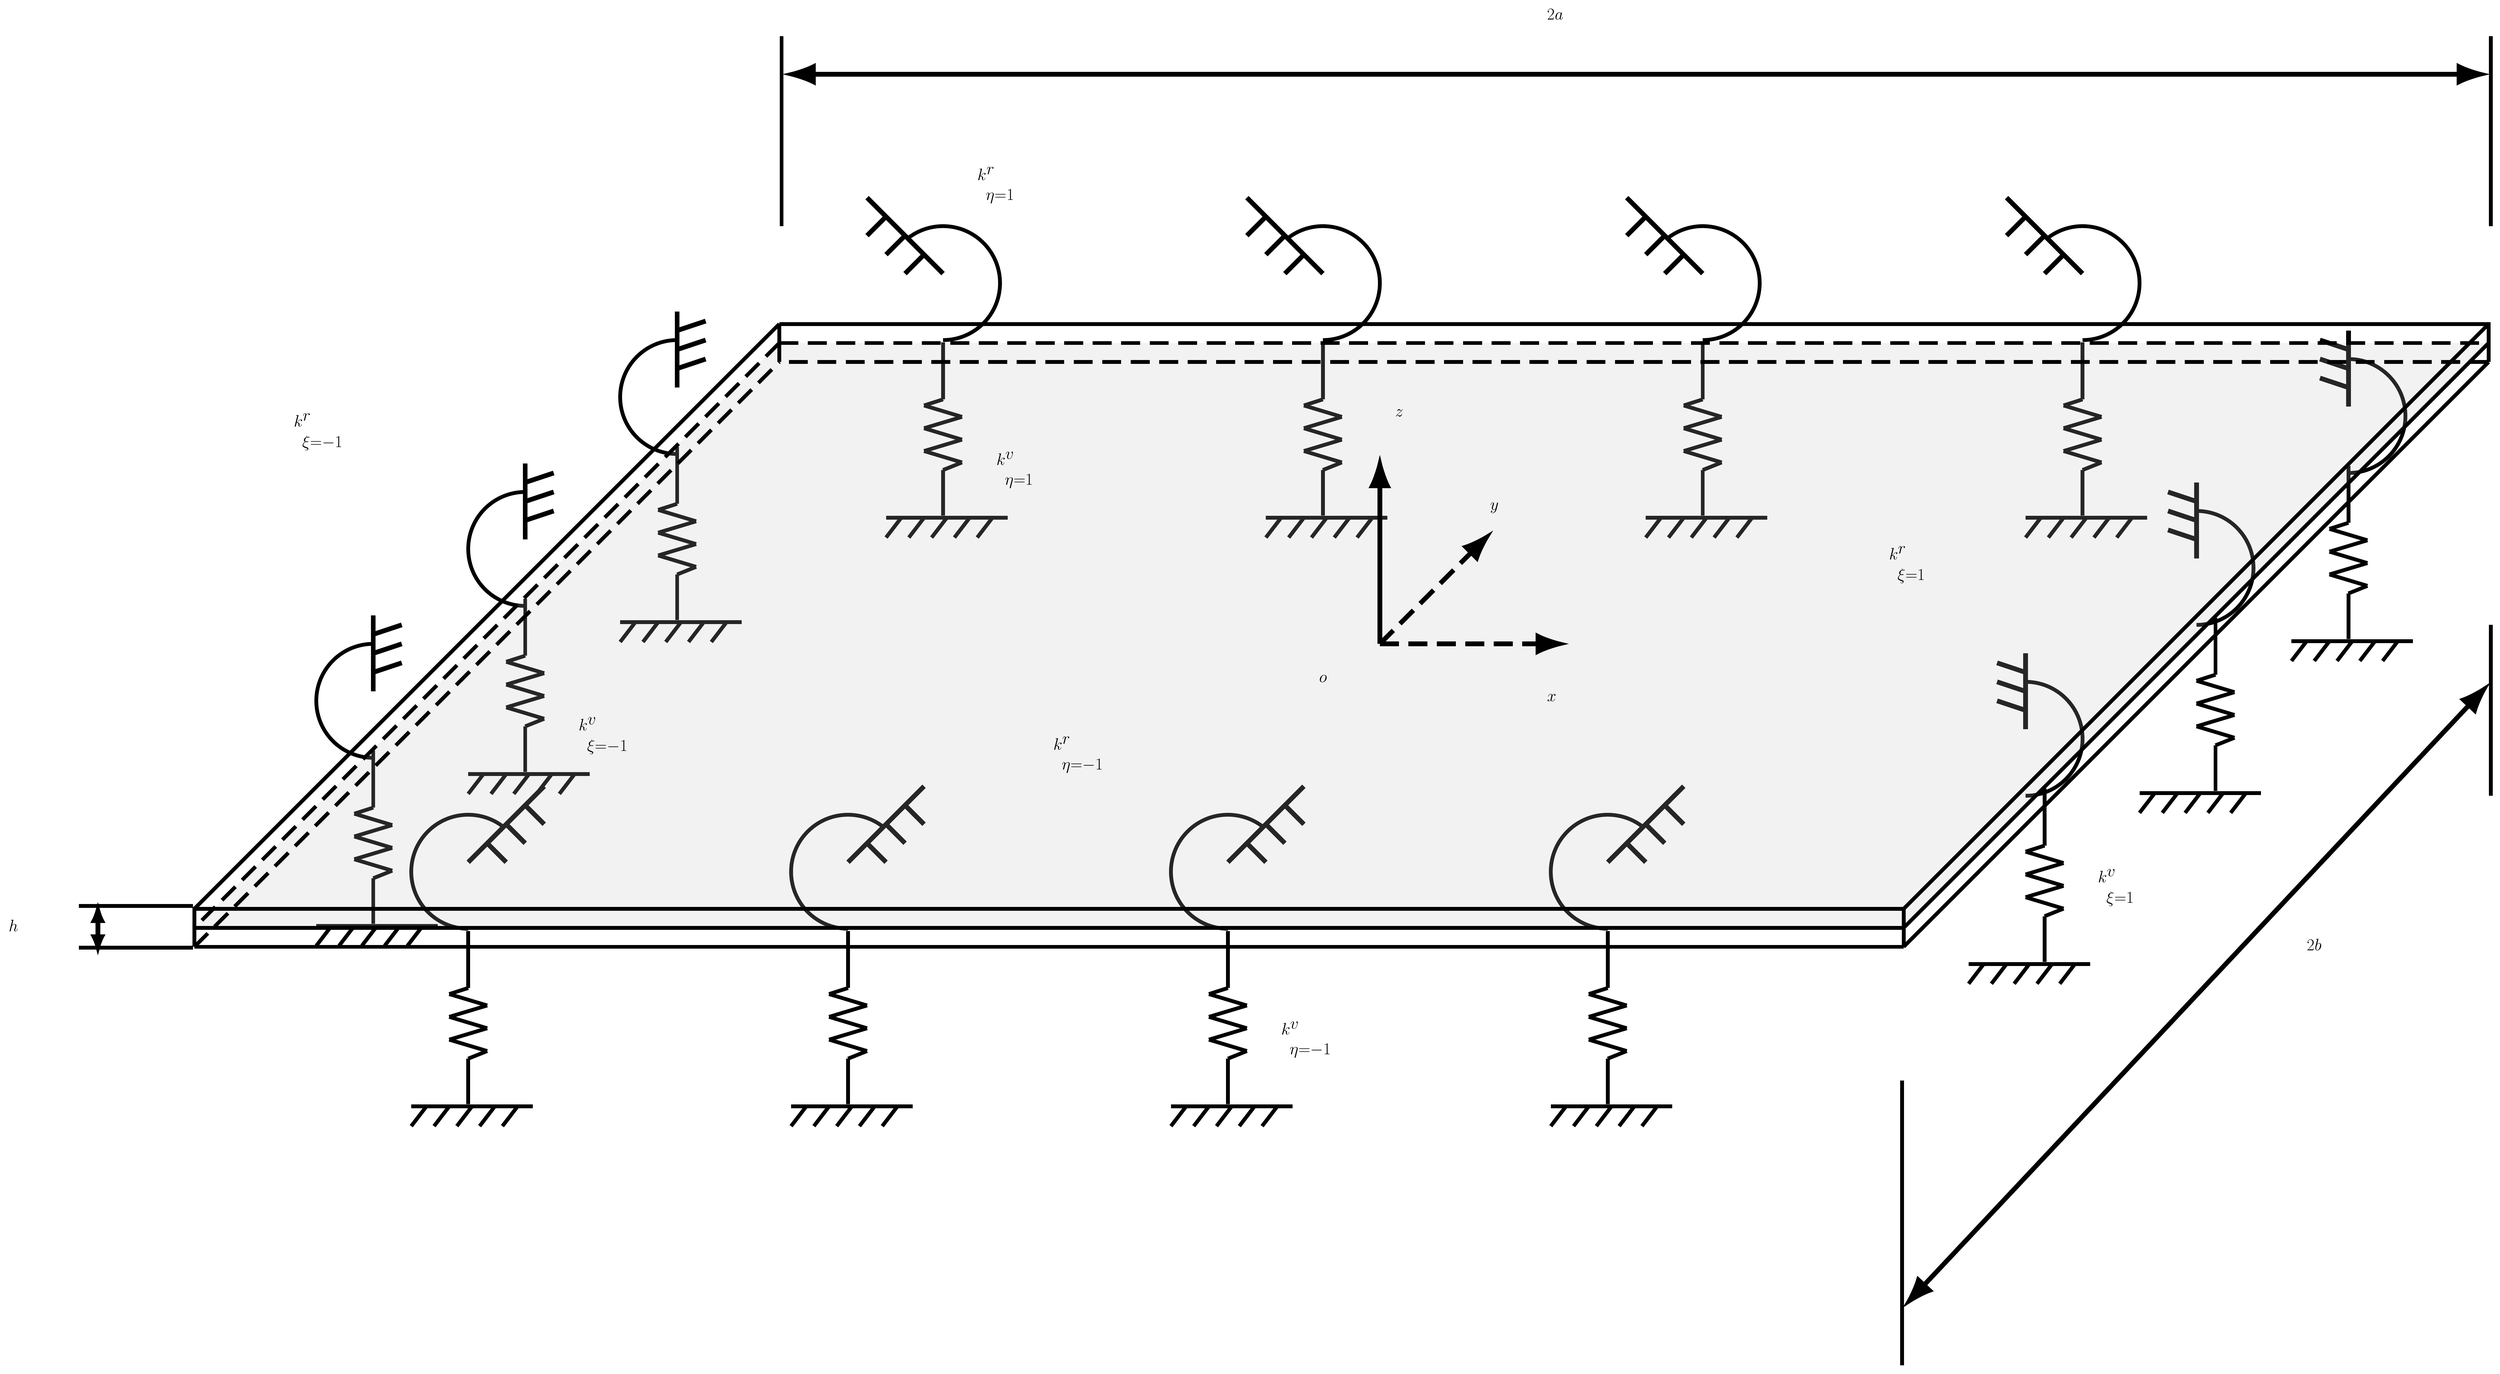
\begin{tikzpicture}[yscale=1]
	\tikzset{
	pics/boundary-box/.style={
		code={
			\begin{scope}[shift={(0mm,0mm)}]
				\definecolor{fc}{RGB}{204,204,204}
				\draw [fill=none, draw=black, line width=0.6mm] (000.0mm,0.0mm)
				-- ++(0.0mm,60.0mm)
				-- ++(-60.0mm,0.0mm)
				-- ++(0.0mm,-60.0mm)  % Adjusted the vertical length to 20mm
				-- ++(60.0mm,0.0mm)  % Adjusted the vertical length to 20mm
				-- cycle;
				\node [black, anchor=west, font=\fontsize{100}{0}\selectfont\bfseries] at (-40mm, 30mm) { $\textbf{?}$ };
			\end{scope}
		}
	}
}
\tikzset{
	pics/Mass-circle/.style={
		code={
			\draw[fill=gray!30, draw=black, line width=0.6mm] (0mm, 0mm) circle [radius=38mm];
		}
	}
}
\tikzset{
	pics/Beam/.style={
		code={\draw [fill=none,draw=black,line width=10.0mm] (000.0mm,0.mm)
			-- ++(600.0mm,0.0mm)
			;
			%% curvature
			\draw[fill=none, draw=gray, line width=4.0mm, dash pattern=on 20pt off 20pt] (000.0mm,0.mm) .. controls (200mm,-100mm) and (300mm,-50mm) .. (600.0mm,0mm);
			
			
		}
	}
}
\tikzset{
	pics/Spring-damp/.style={
		code={\begin{scope}[cm={0.4,0,0,0.4,(40.0mm,0mm)}]
				\draw [fill=none,draw=black,line width=2.0mm] (145.0mm,707.4mm)
				-- ++(0.0mm,33.0mm)
				;
				\draw [fill=none,draw=black,line width=2.0mm] (120.0mm,867.4mm)
				-- ++(50.0mm,-15.0mm)
				;
				\draw [fill=none,draw=black,line width=2.0mm] (170.0mm,852.4mm)
				-- ++(-50.0mm,-15.0mm)
				;
				\draw [fill=none,draw=black,line width=2.0mm] (120.0mm,837.4mm)
				-- ++(50.0mm,-15.0mm)
				;
				\draw [fill=none,draw=black,line width=2.0mm] (170.0mm,822.4mm)
				-- ++(-50.0mm,-15.0mm)
				;
				
				\draw [fill=none,draw=black,line width=2.0mm] (120.0mm,807.4mm)
				-- ++(50.0mm,-15.0mm)
				;
				
				\draw [fill=none,draw=black,line width=2.0mm] (170.0mm,792.4mm)
				-- (120.0mm,777.4mm)
				;
				
				\draw [fill=none,draw=black,line width=2.0mm] (120.0mm,777.4mm)
				-- ++(50.0mm,-15.0mm)
				;
				
				\draw [fill=none,draw=black,line width=2.0mm] (170.0mm,762.4mm)
				-- ++(-50.0mm,-15.0mm)
				;
				
				\draw [fill=none,draw=black,line width=2.0mm] (145.0mm,875.4mm)
				-- ++(-25.0mm,-8.0mm)
				;
				
				\draw [fill=none,draw=black,line width=2.0mm] (120.0mm,747.4mm)
				-- ++(25.0mm,-7.0mm)
				;
				
				\draw [fill=none,draw=black,line width=2.0mm] (145.0mm,875.4mm)
				-- (145.0mm,907.4mm)
				;
			\end{scope}
			% horizontal line above mass left
			\draw [fill=none,draw=black,line width=2.0mm] (58.0mm,363mm)
			-- ++(40.0mm,0.0mm)
			;
			
			%% damping left
			\begin{scope}[cm={0.4,0,0,-0.4,(0.0mm,645.9mm)}]
				\draw [fill=none,draw=black,line width=2.0mm] (115.0mm,827.7mm)
				-- ++(0.0mm,-35.3mm)
				-- (175.0mm,792.4mm)
				-- ++(0.0mm,35.0mm)
				;
				
				\draw [fill=none,draw=black,line width=2.0mm] (145.0mm,707.4mm)
				-- ++(0.0mm,85.0mm)
				;
				
				\draw [fill=none,draw=black,line width=2.0mm] (123.0mm,807.4mm)
				-- ++(44.0mm,0.0mm)
				;
				
				\draw [fill=none,draw=black,line width=2.0mm] (145.0mm,807.4mm)
				-- ++(0.0mm,100.0mm)
				;
			\end{scope}
			
			%% suspension arrow left
			\draw [fill=none,draw=black,line width=2.0mm] (58.0mm,283.4mm)
			-- ++(40.0mm,0.0mm)
			;
			\draw [fill=none,draw=black,line width=2.0mm] (78.0mm,363.4mm)
			-- ++(0mm,27.0mm)
			;
			%% vertical line upp
			\draw [fill=none,draw=black,line width=2.0mm] (78.0mm,283.4mm)
			-- ++(0.0mm,-30.0mm)
			;
		}
	}
}
\tikzset{
	pics/beam-Spring/.style={
		code={\begin{scope}[cm={0.4,0,0,0.4,(-38.0mm,-256.4mm)}]
				\draw [fill=none,draw=black,line width=2.0mm] (145.0mm,782.4mm)
				-- ++(0.0mm,-60.0mm)
				;
				\draw [fill=none,draw=black,line width=2.0mm] (120.0mm,867.4mm)
				-- ++(50.0mm,-15.0mm)
				;
				\draw [fill=none,draw=black,line width=2.0mm] (170.0mm,852.4mm)
				-- ++(-50.0mm,-15.0mm)
				;
				\draw [fill=none,draw=black,line width=2.0mm] (120.0mm,837.4mm)
				-- ++(50.0mm,-15.0mm)
				;
				\draw [fill=none,draw=black,line width=2.0mm] (170.0mm,822.4mm)
				-- ++(-50.0mm,-15.0mm)
				;
				\draw [fill=none,draw=black,line width=2.0mm] (120.0mm,807.4mm)
				-- ++(50.0mm,-15.0mm)
				;
				\draw [fill=none,draw=black,line width=2.0mm] (170.0mm,792.4mm)
				-- (145.0mm,782.4mm)
				;
				
				
			
				\draw [fill=none,draw=black,line width=2.0mm] (145.0mm,875.4mm)
				-- ++(-25.0mm,-8.0mm)
				;
				
				\draw [fill=none,draw=black,line width=2.0mm] (145.0mm,875.4mm)
				-- (145.0mm,950.4mm)
				;
			\end{scope}
			
		}
	}
}
\tikzset{
	pics/beam-arrow/.style={
		code={% bridge curve property 
			\draw [fill=none,draw=black,line width=2.0mm] (380.0mm,32.0mm)
			.. controls ++(85.0mm,-8.0mm) and ++(-60.0mm,-6.0mm) .. ++(135.0mm,-32.0mm)
			;
			%% arraw of bridge curve property 
			\draw [->, black, line width=6mm, >=stealth, shorten >=1pt] (515.0mm,0mm) -- ++(0.5,0); % Draws the arrowhead separately
			
		}
	}
}
\tikzset{
	pics/beam-prop-arrow/.style={
		code={% bridge curve deflection yx
			\draw [fill=none,draw=black,line width=2.0mm] (440.0mm,0.0mm)
			.. controls ++(85.0mm,5.0mm) and ++(-60.0mm,4.0mm) .. ++(135.0mm,36.0mm)
			;
			%% arraw of bridge curve deflection yx
			\draw [black, line width=2mm] (570.0mm,36.0mm) -- (580.0mm,36.0mm);
			\draw [->, black, line width=6mm, >=stealth, shorten >=1pt] (580.0mm,36.0mm) -- ++(0.5,0); % Draws the arrowhead separately
			
		}
	}
}
\tikzset{
	pics/mass-defle/.style={
		code={%% arraw of vehicle deflection yv 
			\draw [->,fill=none,draw=black,line width=2.50mm] (0.0mm,25.0mm)
			-- (30.0mm,25.0mm)
			-- (30.0mm,65.3mm)
			;			
		}
	}
}
\tikzset{
	pics/floor/.style={
		code={
			%  left
			\begin{scope}[cm={0.4,0,0,-0.4,(-42.0mm,377.0mm)}]
				\draw [fill=none,draw=black,line width=2.0mm] (30.0mm,939mm)
				-- (190.0mm,939mm)
				;
				\draw [fill=none,draw=black,line width=2.0mm] (50.0mm,939mm)
				-- (30.0mm,965mm)
				;
				\draw [fill=none,draw=black,line width=2.0mm] (80.0mm,939mm)
				-- (60.0mm,965mm)
				;
				\draw [fill=none,draw=black,line width=2.0mm] (110.0mm,939mm)
				-- (90.0mm,965mm)
				;
				\draw [fill=none,draw=black,line width=2.0mm] (140.0mm,939mm)
				-- (120.0mm,965mm)
				;
				\draw [fill=none,draw=black,line width=2.0mm] (170.0mm,939mm)
				-- (150.0mm,965mm)
				;
			\end{scope}
			
		}
	}
}
\tikzset{
	pics/beam-rotation/.style={
		code={
			%%% arc representing rotation or deflection
			\draw [-,fill=none,draw=black,line width=2.00mm] 
			(0.0mm,25.0mm) arc [start angle=270, end angle=90, radius=30mm];
			\draw [fill=none,draw=black,line width=2.5mm] (0.0mm,60mm)
			-- (0.0mm,100mm)
			;
			
			\draw [fill=none,draw=black,line width=2.5mm] (0.0mm,70mm)
			-- (15.0mm,75mm)
			;
			\draw [fill=none,draw=black,line width=2.5mm] (0.0mm,80mm)
			-- (15.0mm,85mm)
			;
			\draw [fill=none,draw=black,line width=2.5mm] (0.0mm,90mm)
			-- (15.0mm,95mm)
			;
			
		}
	}
}
\tikzset{
	pics/beam-rotation-bot/.style={
		code={
			%%% arc representing rotation or deflection
			\draw [-,fill=none,draw=black,line width=2.00mm] 
			(0.0mm,25.0mm) arc [start angle=270, end angle=50, radius=30mm];
			\draw [fill=none,draw=black,line width=2.5mm] (0.0mm,60mm)
			-- (40.0mm,100mm)
			;
			
			\draw [fill=none,draw=black,line width=2.5mm] (10mm,70mm)
			-- (20.0mm,60mm)
			;
			\draw [fill=none,draw=black,line width=2.5mm] (20mm,80mm)
			-- (30.0mm,70mm)
			;
			\draw [fill=none,draw=black,line width=2.5mm] (30mm,90mm)
			-- (40.0mm,80mm)
			;
			
		}
	}
}
\tikzset{
	pics/Rectangular-Plate/.style={
		code={
			% Define the vertices of the rectangular plate
			\coordinate (A) at (0, 1, 0);
			\coordinate (B) at (90, 1, 0);
			\coordinate (C) at (90, 2, 0);
			\coordinate (D) at (0, 2, 0);
			\coordinate (A') at (0, 1, 80);
			\coordinate (B') at (90, 1, 80);
			\coordinate (C') at (90, 2, 80);
			\coordinate (D') at (0, 2, 80);
			\coordinate (E) at (0, 0, 0);
			\coordinate (F) at (90, 0, 0);
			\coordinate (E') at (0, 0, 80);
			\coordinate (F') at (90, 0, 80);
			
			% Fill the surface AA'B'B with gray and transparent
			\fill[gray!50, fill opacity=0.2] (A) -- (A') -- (B') -- (B) -- cycle;
			
			% Draw the edges of the bottom face
			\draw[black, line width=2mm, dashed, dash pattern=on 10mm off 5mm] (A) -- (B); % AB dashed
			\draw[black, line width=2mm] (B) -- (C) -- (D); % Remaining edges solid
			\draw[black, line width=2mm, dashed, dash pattern=on 10mm off 5mm] (D) -- (A); % AD dashed
			\draw[black, line width=2mm, dashed, dash pattern=on 10mm off 5mm] (A) -- (E); % AB dashed
			\draw[black, line width=2mm, dashed, dash pattern=on 10mm off 5mm] (F) -- (E); % AB dashed
			\draw[black, line width=2mm, dashed, dash pattern=on 10mm off 5mm] (F) -- (B); % AB dashed
			\draw[black, line width=2mm, dashed, dash pattern=on 10mm off 5mm] (E') -- (E); % AB dashed

			% Draw the edges of the top face
			\draw[black, line width=2mm] (A') -- (B') -- (C') -- (D') -- cycle;
			
			% Draw the vertical edges connecting the bottom and top faces
			\draw[black, line width=2mm, dashed, dash pattern=on 10mm off 5mm] (A) -- (A'); % AA' dashed
			\draw[black, line width=2mm] (B) -- (B');
			\draw[black, line width=2mm] (C) -- (C');
			\draw[black, line width=2mm] (D) -- (D');
			\draw[black, line width=2mm] (F) -- (F');
			\draw[black, line width=2mm] (A') -- (E');
			\draw[black, line width=2mm] (B') -- (F');
			\draw[black, line width=2mm] (F') -- (E');
		}
	}
}



	%%%%%%%%%%%%%%%%%%%%%%%%%%%%%%%%% drawing
	%\pic at (700mm,0mm) {boundary-box};
	%\pic at (40mm,0mm) {boundary-box};
	\pic at (20mm,-25mm) {beam-rotation};
	\pic at (0mm,-120mm) {beam-Spring};
	\pic at (20mm,-90mm) {floor};
	\pic at (-60mm,-105mm) {beam-rotation};
	\pic at (-80mm,-200mm) {beam-Spring};
	\pic at (-60mm,-170mm) {floor};
	\pic at (-140mm,-185mm) {beam-rotation};
	\pic at (-160mm,-280mm) {beam-Spring};
	\pic at (-140mm,-250mm) {floor};

	%%%%%%%%%%%%
	\pic[xscale=-1] at (900mm,-35mm) {beam-rotation};
	\pic at (880mm,-130mm) {beam-Spring};
	\pic at (900mm,-100mm) {floor};
	\pic[xscale=-1] at (820mm,-115mm) {beam-rotation};
	\pic at (810mm,-210mm) {beam-Spring};
	\pic at (820mm,-180mm) {floor};
	\pic[xscale=-1] at (730mm,-205mm) {beam-rotation};
	\pic at (720mm,-300mm) {beam-Spring};
	\pic at (730mm,-270mm) {floor};
%%%%%%%%%%%%%%%%%%%%%%%%
	\pic[xscale=-1] at (160mm,35mm) {beam-rotation-bot};
	\pic at (140mm,-65mm) {beam-Spring};
	\pic at (160mm,-35mm) {floor};
	\pic[xscale=-1] at (360mm,35mm) {beam-rotation-bot};
	\pic at (340mm,-65mm) {beam-Spring};
	\pic at (360mm,-35mm) {floor};
	\pic[xscale=-1] at (560mm,35mm) {beam-rotation-bot};
	\pic at (540mm,-65mm) {beam-Spring};
	\pic at (560mm,-35mm) {floor};
	\pic[xscale=-1] at (760mm,35mm) {beam-rotation-bot};
	\pic at (740mm,-65mm) {beam-Spring};
	\pic at (760mm,-35mm) {floor};
	%%%%%%%%%
	\pic[xscale=1] at (510mm,-275mm) {beam-rotation-bot};
	\pic at (490mm,-375mm) {beam-Spring};
	\pic at (510mm,-345mm) {floor};
	\pic[xscale=1] at (310mm,-275mm) {beam-rotation-bot};
	\pic at (290mm,-375mm) {beam-Spring};
	\pic at (310mm,-345mm) {floor};
	\pic[xscale=1] at (110mm,-275mm) {beam-rotation-bot};
	\pic at (90mm,-375mm) {beam-Spring};
	\pic at (110mm,-345mm) {floor};
	\pic[xscale=1] at (-90mm,-275mm) {beam-rotation-bot};
	\pic at (-110mm,-375mm) {beam-Spring};
	\pic at (-90mm,-345mm) {floor};
	
	%%%%%%%%
    \pic at (3mm, 6, 3) {Rectangular-Plate};
    
    %%%%%%%%%%%%%%%%%%%%%
    %%% 2b
    \begin{scope}[shift={(-35mm,-180.0mm)}]
    	\draw[{Latex[length=18mm, width=12mm]}-{Latex[length=18mm, width=12mm]}, fill=none, draw=black, line width=2.5mm] 
    	(700mm,-270.0mm) -- (1010mm,60.0mm);
    	\draw [-,fill=none,draw=black,line width=2.mm] (700mm,-150.0mm)
    	-- (700mm,-300.0mm)
    	;
    	\draw [-,fill=none,draw=black,line width=2.mm] (1010mm,90.0mm)
    	-- (1010mm,000.0mm)
    	;
    \end{scope}
    %%% 2a
    \begin{scope}[shift={(-35mm,150.0mm)}]
    	\draw[{Latex[length=18mm, width=12mm]}-{Latex[length=18mm, width=12mm]}, fill=none, draw=black, line width=2.5mm] 
    	 (110mm,50.0mm)
    	-- (1010mm,50.0mm);
    	\draw [-,fill=none,draw=black,line width=2.mm] (110mm,70.0mm)
    	-- (110mm,-30.0mm)
    	;
    	\draw [-,fill=none,draw=black,line width=2.mm] (1010mm,70.0mm)
    	-- (1010mm,-30.0mm)
    	;
    \end{scope}
        %%% h
    \begin{scope}[shift={(-35mm,150.0mm)}]
    	\draw[{Latex[length=12mm, width=8mm]}-{Latex[length=12mm, width=8mm]}, fill=none, draw=black, line width=2.5mm] 
    	(-250mm,-385.0mm)
    	-- (-250mm,-415.0mm);
    	\draw [-,fill=none,draw=black,line width=2.mm] (-260mm,-388.0mm)
    	-- (-200mm,-388.0mm)
    	;
    	\draw [-,fill=none,draw=black,line width=2.mm] (-260mm,-410.0mm)
    	-- (-200mm,-410.0mm)
    	;
    \end{scope}
     %%% xyz
    \begin{scope}[shift={(30mm,-150.0mm)}]
    	\draw[-{Latex[length=18mm, width=12mm]}, fill=none, draw=black, line width=2.5mm, dashed, dash pattern=on 10mm off 5mm] 
    	(360mm,50.0mm) -- (460mm,50.0mm);
    	\draw[-{Latex[length=18mm, width=12mm]}, fill=none, draw=black, line width=2.5mm] 
    	(360mm, 50.0mm) -- (360mm, 150.0mm); 		
    	\draw[-{Latex[length=18mm, width=12mm]}, fill=none, draw=black, line width=2.5mm, dashed, dash pattern=on 10mm off 5mm] 
    	(360mm, 50.0mm) -- (420mm, 110.0mm);
    	
    	
    \end{scope}
	%%%%%%%%%%%%%%%% text
	
	\begin{scope}[shift={(16.9mm,-8.4mm)}]
		\node [black,anchor=west,font=\fontsize{140}{0}\selectfont] at (340mm,-110mm) { $o$ };
		\node [black,anchor=west,font=\fontsize{140}{0}\selectfont] at (460mm,-120mm) { $x$ };
		\node [black,anchor=west,font=\fontsize{140}{0}\selectfont] at (430mm,-20mm) { $y$ };
		\node [black,anchor=west,font=\fontsize{140}{0}\selectfont] at (380mm,30mm) { $z$ };
		\node [black,anchor=west,font=\fontsize{140}{0}\selectfont] at (460mm,240mm) { $2a$ };
		\node [black,anchor=west,font=\fontsize{140}{0}\selectfont] at (860mm,-250mm) { $2b$ };
		\node [black,anchor=west,font=\fontsize{140}{0}\selectfont] at (-350mm,-240mm) { $h$ };
		\node [black,anchor=west,font=\fontsize{140}{0}\selectfont] at (-50mm,-140mm) { $k^v_{\xi=-1}$ };
		\node [black,anchor=west,font=\fontsize{140}{0}\selectfont] at (-200mm,20mm) { $k^r_{\xi=-1}$ };
		\node [black,anchor=west,font=\fontsize{140}{0}\selectfont] at (750mm,-220mm) { $k^v_{\xi=1}$ };
	    \node [black,anchor=west,font=\fontsize{140}{0}\selectfont] at (640mm,-50mm) { $k^r_{\xi=1}$ };
	    \node [black,anchor=west,font=\fontsize{140}{0}\selectfont] at (320mm,-300mm) { $k^v_{\eta=-1}$ };
		\node [black,anchor=west,font=\fontsize{140}{0}\selectfont] at (200mm,-150mm) { $k^r_{\eta=-1}$ };
		\node [black,anchor=west,font=\fontsize{140}{0}\selectfont] at (170mm,0mm) { $k^v_{\eta=1}$ };
		\node [black,anchor=west,font=\fontsize{140}{0}\selectfont] at (160mm,150mm) { $k^r_{\eta=1}$ };
	\end{scope}
\end{tikzpicture}

}
\caption{\small The orthotropic rectangular plate with all edges elastically restrained.} 
\label{fig:platemode}
\end{figure}
Consider a thin orthotropic rectangular plate of length $2a$ and width $2b$, with all four edges restrained by vertical translational springs \DIFdelbegin \DIFdel{$k^v$ and rotational springs $k^r$}\DIFdelend \DIFaddbegin \DIFadd{$k^{v}_{\xi}$ and $k^{v}_{\eta}$, and rotational springs $k^{r}_{\xi}$ and $k^{r}_{\eta}$}\DIFaddend , as shown in \Cref{fig:platemode}.
The coordinate origin is located at the center of the plate.

\DIFdelbegin \DIFdel{The }\DIFdelend \DIFaddbegin \DIFadd{In the traditional SOV method, the strong-form }\DIFaddend governing differential equation for the free vibration of a thin orthotropic plate is given by \citep{xing2020improved}: 
%
\begin{equation}\label{eq:governing_EOM}
D_{11}\DIFdelbegin \DIFdel{\frac{\partial^4w}{\partial \xi^4} }\DIFdelend \DIFaddbegin \DIFadd{\frac{\partial^4W}{\partial \xi^4} }\DIFaddend + 2D_3\chi^2\DIFdelbegin \DIFdel{\frac{\partial^4w}{\partial \xi^2 \partial \eta^2} }\DIFdelend \DIFaddbegin \DIFadd{\frac{\partial^4W}{\partial \xi^2 \partial \eta^2} }\DIFaddend + D_{22}\chi^4\DIFdelbegin \DIFdel{\frac{\partial^4w}{\partial \eta^4} }\DIFdelend \DIFaddbegin \DIFadd{\frac{\partial^4W}{\partial \eta^4} }\DIFaddend = \rho ha^4\omega^2\DIFdelbegin \DIFdel{w}\DIFdelend \DIFaddbegin \DIFadd{W}\DIFaddend ,
\end{equation}
%
where \DIFaddbegin \DIFadd{$W(\xi,\eta)$ is the mode shape function; }\DIFaddend $ \chi = a / b $ is the aspect ratio; $ \xi = x / a $ and $ \eta = y / b $ are the normalized coordinates, and the bending stiffness parameters are defined as:
%
\begin{equation}\label{eq:bd_stiff}
\begin{split}
	&D_{11} = \DIFdelbegin \DIFdel{\frac{E_1h^3}{12(1-v_{12}v_{21})}}\DIFdelend \DIFaddbegin \DIFadd{\frac{E_1h^3}{12(1-\nu_{12}\nu_{21})}}\DIFaddend , \qquad D_{22} = \DIFdelbegin \DIFdel{\frac{E_2h^3}{12(1-v_{12}v_{21})}}\DIFdelend \DIFaddbegin \DIFadd{\frac{E_2h^3}{12(1-\nu_{12}\nu_{21})}}\DIFaddend , \\  
	&D_{66} = \frac{G_{12}h^3}{12}, \quad D_{12} = \DIFdelbegin \DIFdel{v}\DIFdelend \DIFaddbegin \DIFadd{\nu}\DIFaddend _{12}D_{22} = \DIFdelbegin \DIFdel{v}\DIFdelend \DIFaddbegin \DIFadd{\nu}\DIFaddend _{21}D_{11}, \quad D_3 = D_{12} + 2D_{66},
\end{split}
\end{equation}
%
where $\rho$ and $h$ denote the mass density and thickness of the plate, respectively; $E_1$ and $E_2$ are the Young’s moduli in the $x$- and $y$-directions, respectively; $G_{12}$ is the shear modulus, and \DIFdelbegin \DIFdel{$v_{12}$ and $v_{21}$ }\DIFdelend \DIFaddbegin \DIFadd{$\nu_{12}$ and $\nu_{21}$ }\DIFaddend are the Poisson’s ratios.

\DIFaddbegin \DIFadd{The traditional SOV method is based on the strong-form governing equation in \mbox{%DIFAUXCMD
\Cref{eq:governing_EOM}}\hskip0pt%DIFAUXCMD
, and the details are not given here; more information can be found in \mbox{%DIFAUXCMD
\cite{xing2009new}}\hskip0pt%DIFAUXCMD
. 
However, the traditional SOV method cannot deal with free boundary conditions, thus the extended SOV method is proposed.
}


\subsection{\DIFadd{Mathematical model for extended separation-of-variable method}}\label{sec:esovmodel}

\DIFaddend Instead of solving the free vibration \DIFaddbegin \DIFadd{problem }\DIFaddend of the thin orthotropic plate using \DIFdelbegin \DIFdel{\mbox{%DIFAUXCMD
\Cref{eq:governing_EOM}}\hskip0pt%DIFAUXCMD
, it is suggested }\DIFdelend \DIFaddbegin \DIFadd{the strong-form governing equation in \mbox{%DIFAUXCMD
\Cref{eq:governing_EOM}}\hskip0pt%DIFAUXCMD
, the extended SOV method suggests }\DIFaddend that the vibration \DIFdelbegin \DIFdel{of the thin plate can also be solved using }\DIFdelend \DIFaddbegin \DIFadd{characteristics can alternatively be obtained through }\DIFaddend the Rayleigh quotient variational principle \cite{xing2018overall}\DIFaddbegin \DIFadd{, which is also the formulation adopted in the present paper}\DIFaddend :
%
\begin{equation}\label{eq:Rayleigh}
\begin{split}
	\delta U &= \delta T,
\end{split}
\end{equation}
%
where $\delta$ denotes variation, $U$ is the magnitude of the potential energy of the plate, and $T$ represents the magnitude of the kinetic energy of the plate.
\DIFdelbegin \DIFdel{The }\DIFdelend \DIFaddbegin \DIFadd{It should be noted that the formulation of Rayleigh’s principle used here focuses only on undamped vibration, and the dissipation energy is therefore ignored in this study.
The dissipation energy arising from internal damping \mbox{%DIFAUXCMD
\cite{du2025novel} }\hskip0pt%DIFAUXCMD
within the plate could contribute to the governing differential equations of the plate,
while the effects of external damping \mbox{%DIFAUXCMD
\cite{svedholm2016vibration} }\hskip0pt%DIFAUXCMD
could contribute to the transcendental equations corresponding to the boundary conditions.
The application of such damping mechanisms is beyond the scope of the present study, but provides a meaningful direction for future research.
The }\DIFaddend potential energy of the plate can be expressed as \cite{xing2020extended}:
%
\begin{equation}\label{eq:poten_energy}
\begin{split}
	U^{I} &= \frac{1}{2}\iint \Bigg[D_{11}\left(\DIFdelbegin \DIFdel{\frac{\partial^2 W}{\partial x^2}}\DIFdelend \DIFaddbegin \DIFadd{\frac{\partial^2 w}{\partial x^2}}\DIFaddend \right)^2 + 2D_{12}\DIFdelbegin \DIFdel{\frac{\partial^2 W}{\partial x^2}\frac{\partial^2 W}{\partial y^2} }\DIFdelend \DIFaddbegin \DIFadd{\frac{\partial^2 w}{\partial x^2}\frac{\partial^2 w}{\partial y^2} }\DIFaddend + D_{22}\left(\DIFdelbegin \DIFdel{\frac{\partial^2 W}{\partial y^2}}\DIFdelend \DIFaddbegin \DIFadd{\frac{\partial^2 w}{\partial y^2}}\DIFaddend \right)^2 \\
	&\qquad + 4D_{66}\left(\DIFdelbegin \DIFdel{\frac{\partial^2 W}{\partial x \partial y}}\DIFdelend \DIFaddbegin \DIFadd{\frac{\partial^2 w}{\partial x \partial y}}\DIFaddend \right)^2\Bigg] \, \mathrm{d}x \, \mathrm{d}y.
\end{split}
\end{equation}
%
And the kinetic energy is:
%
\begin{equation}\label{eq:kine_energy}
\begin{split}
	T &= \frac{1}{2}\iint \rho h \left(\DIFdelbegin \DIFdel{\frac{\partial W}{\partial t}}\DIFdelend \DIFaddbegin \DIFadd{\frac{\partial w}{\partial t}}\DIFaddend \right)^2 \, \mathrm{d}x \, \mathrm{d}y.
\end{split}
\end{equation}

Assuming the solution of the deflection \DIFdelbegin \DIFdel{$ W(x, y; t) = w(x, y) e^{i \omega t} $ }\DIFdelend \DIFaddbegin \DIFadd{$ w(x, y; t) = W(x, y) e^{i \omega t} $ }\DIFaddend for harmonic plate motion, 
where $ \ii = \sqrt{-1} $, \DIFdelbegin \DIFdel{$ w(x, y) $ }\DIFdelend \DIFaddbegin \DIFadd{$ W(x, y) $ }\DIFaddend is the mode shape, and $ \omega $ is the radial frequency.  
By substituting \DIFdelbegin \DIFdel{$ W(x, y; t) = w(x, y) e^{i \omega t} $ }\DIFdelend \DIFaddbegin \DIFadd{$ w(x, y; t) = W(x, y) e^{i \omega t} $ }\DIFaddend into \Cref{eq:poten_energy,eq:kine_energy} and expressing the system in dimensionless coordinates, we have:
%
\begin{equation}\label{eq:poten_energy_mag}
\begin{split}
	U^{I} &= \frac{ab}{2} \iint \left[ \frac{D_{11}}{a^4} \left( \DIFdelbegin \DIFdel{\frac{\partial^2 w}{\partial \xi^2} }\DIFdelend \DIFaddbegin \DIFadd{\frac{\partial^2 W}{\partial \xi^2} }\DIFaddend \right)^2 + \frac{2 D_{12}}{a^2 b^2} \DIFdelbegin \DIFdel{\frac{\partial^2 w}{\partial \xi^2} \frac{\partial^2 w}{\partial \eta^2} }\DIFdelend \DIFaddbegin \DIFadd{\frac{\partial^2 W}{\partial \xi^2} \frac{\partial^2 W}{\partial \eta^2} }\DIFaddend + \frac{D_{22}}{b^4} \left( \DIFdelbegin \DIFdel{\frac{\partial^2 w}{\partial \eta^2} }\DIFdelend \DIFaddbegin \DIFadd{\frac{\partial^2 W}{\partial \eta^2} }\DIFaddend \right)^2 \right. \\
	&\quad \left. + \frac{4 D_{66}}{a^2 b^2} \left( \DIFdelbegin \DIFdel{\frac{\partial^2 w}{\partial \xi \partial \eta} }\DIFdelend \DIFaddbegin \DIFadd{\frac{\partial^2 W}{\partial \xi \partial \eta} }\DIFaddend \right)^2 \right] \, \mathrm{d} \xi \, \mathrm{d} \eta,
\end{split}
\end{equation}
%
and
%
\begin{equation}\label{eq:kine_energy_mag}
\begin{split}
	T &= \omega^2 \frac{ab}{2} \rho h \iint \DIFdelbegin \DIFdel{w}\DIFdelend \DIFaddbegin \DIFadd{W}\DIFaddend ^2 \, \mathrm{d} \xi \, \mathrm{d} \eta=\omega^2T_0
\end{split},
\end{equation}
%
where, $T_0$ is defined as the coefficient of the kinetic energy.

The separable form of the mode shape function $ w(\xi, \eta)$ is given by:
%
\begin{equation}\label{eq:displace_func}
\DIFdelbegin \DIFdel{w}\DIFdelend \DIFaddbegin \DIFadd{W}\DIFaddend (\xi, \eta) = \phi(\xi) \psi(\eta),
\end{equation}
%
where $ \phi(\xi) $ and $\psi(\eta) $ can be expressed as:
\begin{subequations}\label{eq:phi_psi_solution}
\begin{align}
	\phi(\xi) &= A_1 \sin{(\alpha_1 \xi)} + A_2 \cos{(\alpha_1 \xi)} + A_3 \sinh{(\beta_1 \xi)} + A_4 \cosh{(\beta_1 \xi)},\label{eq:phi_solution1}\\
	\psi(\eta) &= B_1 \sin{(\alpha_2 \eta)} + B_2 \cos{(\alpha_2 \eta)} + B_3 \sinh{(\beta_2 \eta)} + B_4 \cosh{(\beta_2 \eta)}. \label{eq:phi_solution2}
\end{align}
\end{subequations}

\DIFdelbegin \DIFdel{Based on \mbox{%DIFAUXCMD
\Cref{eq:Rayleigh}}\hskip0pt%DIFAUXCMD
, the frequencies }\DIFdelend \DIFaddbegin \DIFadd{In the extended SOV method, by assuming the mode shape $\psi(\eta)$ corresponding to the $y$-direction is known, then we can get the governing differential equation from Rayleigh principle \mbox{%DIFAUXCMD
\Cref{eq:Rayleigh} }\hskip0pt%DIFAUXCMD
in the $x$-direction with the corresponding frequency }\DIFaddend $\omega_x$\DIFdelbegin \DIFdel{and $\omega_y$, corresponding to the mode shapes }\DIFdelend \DIFaddbegin \DIFadd{, and in this case the Rayleigh principle is written in the form in \mbox{%DIFAUXCMD
\Cref{eq:Rayleighx}}\hskip0pt%DIFAUXCMD
. 
Similarly, by assuming the mode shape }\DIFaddend $\phi(\xi)$ \DIFaddbegin \DIFadd{is known, we can get another governing differential equation from \mbox{%DIFAUXCMD
\Cref{eq:Rayleigh} }\hskip0pt%DIFAUXCMD
in the $y$-direction with the corresponding frequency $\omega_y$, and in this case the Rayleigh principle is written in the form in \mbox{%DIFAUXCMD
\Cref{eq:Rayleighy}}\hskip0pt%DIFAUXCMD
. 
It should be noted that $\omega_x$ }\DIFaddend and \DIFdelbegin \DIFdel{$\psi(\eta)$, respectively, }\DIFdelend \DIFaddbegin \DIFadd{$\omega_y$ }\DIFaddend are assumed to be independent of each other \DIFdelbegin \DIFdel{.
This is a common and important assumption in SOV methods, and $\omega_x$ }\DIFdelend and \DIFdelbegin \DIFdel{$\omega_y$ }\DIFdelend can be different in a mathematical sense \DIFdelbegin \DIFdel{\mbox{%DIFAUXCMD
\cite{xing2020extended}}\hskip0pt%DIFAUXCMD
. 
}\DIFdelend \DIFaddbegin \DIFadd{in the extended SOV method \mbox{%DIFAUXCMD
\citep{xing2020extended}}\hskip0pt%DIFAUXCMD
. 
The SOV formulation used in the present work bases on this extended SOV method, and more details of the derivation will be given in the following.
}\DIFaddend 

\subsection{Dynamic stiffness matrix corresponding to $\omega_x$}\label{sec:DSMx}
For given general homogeneous boundary conditions, we can first assume that the mode shape $\psi(\eta)$ corresponding to the $y$-direction is known. 
Supposing the edges of the plate in both the $x$- and $y$-directions are elastically restrained by homogeneous vertical translational and rotational springs.
The vertical translational and rotational springs at the $\xi = -1$ end are denoted as $k^v_{\xi = -1}$ and $k^r_{\xi = -1}$, respectively, and at the $\xi = 1$ end as $k^v_{\xi = 1}$ and $k^r_{\xi = 1}$, respectively. 
Thus, the potential energy along the supported edge in the $x$-direction can be expressed by:
%
\begin{equation}\label{eq:poten_energy_edgex}
\begin{split}
	U^{x} &=  \int\left[k^r_{\xi=-1} \left( \DIFdelbegin \DIFdel{\frac{\partial W}{\partial x} }\DIFdelend \DIFaddbegin \DIFadd{\frac{\partial w}{\partial x} }\DIFaddend \right)^2 + k^v_{\xi=-1} \left( \DIFdelbegin \DIFdel{W }\DIFdelend \DIFaddbegin \DIFadd{w }\DIFaddend \right)^2\right]_{x=-a} \id y\\
	&\qquad +  \int\left[k^r_{\xi=1} \left( \DIFdelbegin \DIFdel{\frac{\partial W}{\partial x} }\DIFdelend \DIFaddbegin \DIFadd{\frac{\partial w}{\partial x} }\DIFaddend \right)^2 + k^v_{\xi=1} \left( \DIFdelbegin \DIFdel{W }\DIFdelend \DIFaddbegin \DIFadd{w }\DIFaddend \right)^2\right]_{x=a} \id y.
\end{split}
\end{equation}
%
From \Cref{eq:poten_energy_edgex}, the magnitude of potential energy along the plate edges in the $x$-direction, expressed in dimensionless coordinates, is obtained as:

%
\begin{equation}\label{eq:poten_energy_edgex2}
\begin{split}
	U^{x} &= ab \int\left[\frac{k^r_{\xi=-1}}{a^3} \left( \DIFdelbegin \DIFdel{\frac{\partial w}{\partial \xi} }\DIFdelend \DIFaddbegin \DIFadd{\frac{\partial W}{\partial \xi} }\DIFaddend \right)^2 + \frac{k^v_{\xi=-1}}{a} \left( \DIFdelbegin \DIFdel{w }\DIFdelend \DIFaddbegin \DIFadd{W }\DIFaddend \right)^2\right]_{\xi=-1} \, \id \eta \\
	&\qquad + ab \int\left[\frac{k^r_{\xi=1}}{a^3} \left( \DIFdelbegin \DIFdel{\frac{\partial w}{\partial \xi} }\DIFdelend \DIFaddbegin \DIFadd{\frac{\partial W}{\partial \xi} }\DIFaddend \right)^2 + \frac{k^v_{\xi=1}}{a} \left( \DIFdelbegin \DIFdel{w }\DIFdelend \DIFaddbegin \DIFadd{W }\DIFaddend \right)^2\right]_{\xi=1} \, \id \eta.
\end{split}
\end{equation}
%
The magnitude of total potential energy of the plate in the $x$-direction can be obtained from \Cref{eq:poten_energy_mag,eq:poten_energy_edgex2} as:
%
\begin{equation}\label{eq:poten_energy_tolx}
\begin{split}
	U &= U^{I} + U^{x} \\
	&= \frac{ab}{2} \iint \left[ \frac{D_{11}}{a^4} \left( \DIFdelbegin \DIFdel{\frac{\partial^2 w}{\partial \xi^2} }\DIFdelend \DIFaddbegin \DIFadd{\frac{\partial^2 W}{\partial \xi^2} }\DIFaddend \right)^2 + \frac{2 D_{12}}{a^2 b^2} \DIFdelbegin \DIFdel{\frac{\partial^2 w}{\partial \xi^2} \frac{\partial^2 w}{\partial \eta^2} }\DIFdelend \DIFaddbegin \DIFadd{\frac{\partial^2 W}{\partial \xi^2} \frac{\partial^2 W}{\partial \eta^2} }\DIFaddend + \frac{D_{22}}{b^4} \left( \DIFdelbegin \DIFdel{\frac{\partial^2 w}{\partial \eta^2} }\DIFdelend \DIFaddbegin \DIFadd{\frac{\partial^2 W}{\partial \eta^2} }\DIFaddend \right)^2 \right. \\
	&\qquad \left.  + \frac{4 D_{66}}{a^2 b^2} \left( \DIFdelbegin \DIFdel{\frac{\partial^2 w}{\partial \xi \partial \eta} }\DIFdelend \DIFaddbegin \DIFadd{\frac{\partial^2 W}{\partial \xi \partial \eta} }\DIFaddend \right)^2 \right] \, \id\xi \, \id\eta \\
	&\qquad + ab \int \left[\frac{k^r_{\xi=1}}{a^3} \left( \DIFdelbegin \DIFdel{\frac{\partial w}{\partial \xi} }\DIFdelend \DIFaddbegin \DIFadd{\frac{\partial W}{\partial \xi} }\DIFaddend \right)^2 + \frac{k^v_{\xi=1}}{a} \left( \DIFdelbegin \DIFdel{w }\DIFdelend \DIFaddbegin \DIFadd{W }\DIFaddend \right)^2 \right]_{\xi=1} \, \id \eta \\
	&\qquad + ab \int \left[\frac{k^r_{\xi=-1}}{a^3} \left( \DIFdelbegin \DIFdel{\frac{\partial w}{\partial \xi} }\DIFdelend \DIFaddbegin \DIFadd{\frac{\partial W}{\partial \xi} }\DIFaddend \right)^2 + \frac{k^v_{\xi=-1}}{a} \left( \DIFdelbegin \DIFdel{w }\DIFdelend \DIFaddbegin \DIFadd{W }\DIFaddend \right)^2 \right]_{\xi=-1} \, \id \eta
\end{split}
\end{equation}
%
By substituting \Cref{eq:displace_func} into \Cref{eq:poten_energy_tolx}, we have:
%
\begin{equation}\label{eq:poten_energy_tolx2}
\begin{split}
	U&=\frac{ab}{2} \int_{-1}^{1} \left[ \frac{D_{11}}{a^4}I_1 \left( \frac{\id^2\phi }{\id \xi^2} \right)^2 + \frac{2 D_{12}}{a^2 b^2}I_2 \frac{\id^2\phi }{\id \xi^2}\phi  + \frac{D_{22}}{b^4}I_4  \phi^2 \right. \\
	&\qquad \left. + \frac{4 D_{66}}{a^2 b^2}I_3 \left( \frac{\id \phi }{\id \xi}\right)^2 \right] \, \id\xi \\
	&\qquad + abI_1 \left[\frac{k^r_{\xi=-1}}{a^3} \left( \frac{\id \phi}{\id \xi} \right)^2+ \frac{k^v_{\xi=-1}}{a} \left( \phi \right)^2\right]_{\xi=-1}\\
	&\qquad + abI_1 \left[\frac{k^r_{\xi=1}}{a^3} \left( \frac{\id \phi}{\id \xi} \right)^2+ \frac{k^v_{\xi=1}}{a} \left( \phi \right)^2\right]_{\xi=1},
\end{split}
\end{equation}
%
where the integral parameters $I_1$, $I_2$, $I_3$, and $ I_4$ are defined and expressed in \Cref{sec:appendA}.


By taking \Cref{eq:displace_func} into account, the coefficient $T_0$ of the kinetic energy from \Cref{eq:kine_energy_mag} for the plate in the $x$-direction can be expressed as:
%
\begin{equation}\label{eq:kine_energyx}
\begin{split}
	T_0 = \frac{ab}{2}\rho h\iint \DIFdelbegin \DIFdel{w}\DIFdelend \DIFaddbegin \DIFadd{W}\DIFaddend ^2 \, \id \xi \, \id \eta = \frac{ab}{2}\rho h I_1\int_{-1}^{1} \phi^2 \, \id \xi.
\end{split}
\end{equation}

Taking the Rayleigh principle in the form:
%
\begin{equation}\label{eq:Rayleighx}
\begin{split}
	\delta U &= \omega_x^2 \, \delta T_0,
\end{split}
\end{equation}
%
and by substituting \Cref{eq:poten_energy_tolx2,eq:kine_energyx} into \Cref{eq:Rayleighx}, and relieving $\delta \phi$ and $\delta\frac{\id  \phi}{\id \xi}$ in \Cref{eq:Rayleighx} by calculus of variations, yields:
%
\begin{equation}\label{eq:Rayleighx2}
\begin{split}
	0 &= \int_{-1}^{1} \bigg[ \frac{D_{11}}{a^4} I_1 \frac{\id^4 \phi}{\id \xi^4} 
	+ \bigg( \frac{2D_{12}}{a^2b^2} I_2 - \frac{4D_{66}}{a^2b^2} I_3 \bigg) \frac{\id^2 \phi}{\id \xi^2} \\
	&\qquad + \bigg( \frac{D_{22}}{b^4} I_4 - \omega_x^2 \rho h I_1 \bigg) \phi \bigg] \delta \phi \, \id \xi \\
	&\qquad + \frac{2k^v_{\xi=-1}}{a} I_1 \big(\phi\, \delta \phi\big)_{\xi=-1} 
	+ \frac{2k^v_{\xi=1}}{a} I_1 \big(\phi\, \delta \phi\big)_{\xi=1} \\
	&\qquad + \bigg[ \bigg( \frac{4D_{66}}{a^2b^2} I_3 - \frac{D_{12}}{a^2b^2} I_2 \bigg) \frac{\id \phi}{\id \xi} 
	- \frac{D_{11}}{a^4} I_1 \frac{\id^3 \phi}{\id \xi^3} \bigg] \delta \phi \Big|^{\xi=1}_{\xi=-1} \\
	&\qquad + \bigg( \frac{D_{12}}{a^2b^2} I_2 \phi + \frac{D_{11}}{a^4} I_1 \frac{\id^2 \phi}{\id \xi^2} \bigg) 
	\delta\frac{\id  \phi}{\id \xi} \Big|^{\xi=1}_{\xi=-1} \\
	&\qquad + \frac{2k^r_{\xi=-1}}{a^3} I_1 \bigg(\frac{\id \phi}{\id \xi}\delta \frac{\id \phi}{\id \xi}\bigg)_{\xi=-1} 
	+ \frac{2k^r_{\xi=1}}{a^3} I_1 \bigg(\frac{\id \phi}{\id \xi} \delta\frac{\id \phi}{\id \xi}\bigg)_{\xi=1}.
\end{split}
\end{equation}
%
Thus, the governing differential equation in the $ x $-direction can be obtained from the integration part of \Cref{eq:Rayleighx2} as:
%
\begin{equation}\label{eq:ODEx}
\frac{\id^4 \phi}{\id \xi^4}+ 2\chi^2\left(\frac{D_{12}I_2}{D_{11}I_1}-2\frac{D_{66}I_3}{D_{11}I_1}\right)\frac{\id^2 \phi}{\id \xi^2}+\left(\chi^4\frac{D_{22}I_4}{D_{11}I_1}-a^4\Omega_x^4\right)\phi=0,
\end{equation}
%
where $\Omega_x = \sqrt[4]{\omega_x^2 \rho h / D_{11}}$.
By substituting $\phi(\xi) = A e^{\mu \xi}$ into \Cref{eq:ODEx}, we obtain:
%
\begin{equation}\label{eq:ODEx2}
\begin{split}
	\mu^4 + 2\chi^2\left(\frac{D_{12}I_2}{D_{11}I_1}-2\frac{D_{66}I_3}{D_{11}I_1}\right)\mu^2 + \left(\chi^4\frac{D_{22}I_4}{D_{11}I_1}-a^4\Omega_x^4\right) = 0.
\end{split}
\end{equation}
%
And so the solution for $\mu$ can be expressed as:
%
\begin{equation}\label{eq:mu}
\begin{split}
	\mu_{1,2} = \pm\textit{i} \alpha_1, \qquad \mu_{3,4} = \pm \beta_1,
\end{split}
\end{equation}
%
where,
%
\begin{subequations}\label{eq:alphax}
\begin{align}
	\alpha_1 &= \chi \sqrt{\sqrt{\left(\frac{D_{12}I_2}{D_{11}I_1}-2\frac{D_{66}I_3}{D_{11}I_1}\right)^2 - \frac{D_{22}I_4}{D_{11}I_1} + b^4\Omega_x^4} + \frac{D_{12}I_2}{D_{11}I_1} - 2\frac{D_{66}I_3}{D_{11}I_1}},\label{eq:alphax1}\\
	\beta_1 &= \chi \sqrt{\sqrt{\left(\frac{D_{12}I_2}{D_{11}I_1}-2\frac{D_{66}I_3}{D_{11}I_1}\right)^2 - \frac{D_{22}I_4}{D_{11}I_1} + b^4\Omega_x^4} - \frac{D_{12}I_2}{D_{11}I_1} + 2\frac{D_{66}I_3}{D_{11}I_1}}.\label{eq:alphax2}
\end{align}
\end{subequations}
%
The boundary conditions along the edges in the $x$-direction can be obtained from the remaining $\delta \phi$ and $\delta \frac{\id \phi}{\id \xi}$ parts in \Cref{eq:Rayleighx2}. 
The shear force equilibrium can be obtained from the $\delta \phi$ part:
%
\begin{equation}\label{eq:inertial_forcex}
\begin{split}
	&\left[ \left( \frac{4D_{66}}{a^2b^2} I_3 - \frac{D_{12}}{a^2b^2} I_2 \right) \frac{\id \phi}{\id \xi} 
	- \frac{D_{11}}{a^4} I_1 \frac{\id^3 \phi}{\id \xi^3} \right] \Big|^{\xi=1}_{\xi=-1}\\
	&\quad\qquad+ \frac{2k^v_{\xi=-1}}{a} I_1 \left(\phi\right)_{\xi=-1}
	+ \frac{2k^v_{\xi=1}}{a} I_1 \left(\phi\right)_{\xi=1} = 0,
\end{split}
\end{equation}
%
and from the $\delta \frac{\id \phi}{\id \xi}$ part, the bending moment equilibrium is:
%
\begin{equation}\label{eq:inertial_forcex2}
\begin{split}	
	&\left( \frac{D_{12}}{a^2b^2} I_2 \phi + \frac{D_{11}}{a^4} I_1 \frac{\partial^2 \phi}{\partial \xi^2} \right) 
	\Big|^{\xi=1}_{\xi=-1} \\
	&\qquad + \frac{2k^r_{\xi=-1}}{a^3} I_1 \left(\frac{\partial \phi}{\partial \xi}\right)_{\xi=-1}
	+ \frac{2k^r_{\xi=1}}{a^3} I_1 \left(\frac{\partial \phi}{\partial \xi}\right)_{\xi=1} = 0.
\end{split}
\end{equation}
%
Thus, we can obtain the shear force and bending moment equilibrium along the edges $\xi = -1$ and $\xi = 1$ from \Cref{eq:inertial_forcex,eq:inertial_forcex2}, respectively, as:
%
\begin{subequations}\label{eq:boundaryx}
\begin{align}
	&  \frac{\id^3 \phi}{\id \xi^3} - \chi^2\left( \frac{4D_{66}I_3}{D_{11}I_1}  - \frac{D_{12}I_2}{D_{11}I_1}  \right) \frac{\id \phi}{\id \xi} 
	+\frac{2a^3k^v_{\xi=-1}}{D_{11}}\phi = 0, \quad &\xi = -1, \\
	& \frac{\id^2 \phi}{\id \xi^2} + \frac{\chi^2 D_{12} I_2}{D_{11} I_1} \phi - \frac{2a k^r_{\xi=-1}}{D_{11}} \frac{\id \phi}{\id \xi} = 0, \quad &\xi = -1, \\
	& \frac{\id^3 \phi}{\id \xi^3} - \chi^2\left( \frac{4D_{66}I_3}{D_{11}I_1}  - \frac{D_{12}I_2}{D_{11}I_1}  \right) \frac{\id \phi}{\id \xi} 
	-\frac{2a^3 k^v_{\xi=1}}{D_{11}} \phi = 0, \quad &\xi = 1, \\
	& \frac{\id^2 \phi}{\id \xi^2} + \frac{\chi^2 D_{12} I_2}{D_{11} I_1} \phi + \frac{2a k^r_{\xi=1}}{D_{11}} \frac{\id \phi}{\id \xi} = 0, \quad &\xi = 1.
\end{align}
\end{subequations}

Substituting \Cref{eq:phi_solution1} into \Cref{eq:boundaryx}, and denoting 
$k^{v*}_{\xi} \equiv \frac{2a^3 k^v_{\xi}}{D_{11}} $, 
$ k^{r*}_{\eta} \equiv \frac{2a k^r_{\xi}}{D_{11}} $, 
$ S_{\alpha_1} \equiv \sin \alpha_1 $, 
$ C_{\alpha_1} \equiv \cos \alpha_1 $, 
$ Sh_{\beta_1} \equiv \sinh \beta_1$, 
and $ Ch_{\beta_1} \equiv \cosh \beta_1 $, we have:
%
\begin{equation}\label{eq:ABx}
\begin{split}
	&\left[ \begin{array}{c}
		\gamma_1 C_{\alpha_1} - k^{v*}_{\xi=-1} S_{\alpha_1} \\ 
		\gamma_3 S_{\alpha_1} + k^{r*}_{\xi=-1} \alpha_1 C_{\alpha_1} \\ 
		-\gamma_1 C_{\alpha_1} + k^{v*}_{\xi=1} S_{\alpha_1} \\ 
		\gamma_3 S_{\alpha_1} + k^{r*}_{\xi=1} \alpha_1 C_{\alpha_1}
	\end{array} 
	\begin{array}{c}
		\gamma_1 S_{\alpha_1} + k^{v*}_{\xi=-1} C_{\alpha_1} \\ 
		-\gamma_3 C_{\alpha_1} + k^{r*}_{\xi=-1} \alpha_1 S_{\alpha_1} \\ 
		\gamma_1 S_{\alpha_1} + k^{v*}_{\xi=1} C_{\alpha_1} \\ 
		\gamma_3 C_{\alpha_1} - k^{r*}_{\xi=1} \alpha_1 S_{\alpha_1}
	\end{array} 
	\begin{array}{c}
		\gamma_2 Ch_{\beta_1} - k^{v*}_{\xi=-1} Sh_{\beta_1} \\ 
		\gamma_4 Sh_{\beta_1} + k^{r*}_{\xi=-1} \beta_1 Ch_{\beta_1} \\ 
		-\gamma_2 Ch_{\beta_1} + k^{v*}_{\xi=1} Sh_{\beta_1} \\ 
		\gamma_4 Sh_{\beta_1} + k^{r*}_{\xi=1} \beta_1 Ch_{\beta_1}
	\end{array} \right. \\ 
	&\quad
	\left. \begin{array}{c}
		-\gamma_2 Sh_{\beta_1} + k^{v*}_{\xi=-1} Ch_{\beta_1} \\ 
		-\gamma_4 Ch_{\beta_1} - k^{r*}_{\xi=-1} \beta_1 Sh_{\beta_1} \\ 
		-\gamma_2 Sh_{\beta_1} + k^{v*}_{\xi=1} Ch_{\beta_1} \\ 
		\gamma_4 Ch_{\beta_1} + k^{r*}_{\xi=1} \beta_1 Sh_{\beta_1}
	\end{array} \right] \begin{Bmatrix}
		A_1 \\ A_2 \\ A_3 \\ A_4
	\end{Bmatrix} =  \begin{Bmatrix}
		0 \\ 0 \\ 0 \\ 0
	\end{Bmatrix},
\end{split}
\end{equation}
%
or,
%
\begin{equation}\label{eq:ABx1}
\mathbf{R}_x \mathbf{A} = \mathbf{0},
\end{equation}
%
where,
%
\begin{equation}\label{eq:gamma}
\begin{split}
	&\gamma_1 = -\alpha_1^3 - \chi^2 \left( \frac{4D_{66}S_3}{D_{11}I_1} - \frac{D_{12}I_2}{D_{11}I_1} \right) \alpha_1, \\
	&\gamma_2 = \beta_1^3 - \chi^2 \left( \frac{4D_{66}S_3}{D_{11}I_1} - \frac{D_{12}I_2}{D_{11}I_1} \right) \beta_1, \\
	&\gamma_3 = -\alpha_1^2 + \frac{\chi^2 D_{12} I_2}{D_{11} I_1}, \\
	&\gamma_4 = \beta_1^2 + \frac{\chi^2 D_{12} I_2}{D_{11} I_1}.
\end{split}
\end{equation}

Note that the classic boundary conditions can be obtained by selecting extremely large or small spring stiffness constants.
For non-trivial solutions, the characteristic equation or eigenvalue equation is obtained from the determinant of the matrix $\mathbf{R}_x$ in \Cref{eq:ABx1}, which must be zero.
However, solving these transcendental equations is cumbersome and so the DSM is introduced to avoid such a computation.

To develop the plate's dynamic stiffness matrix, with the help of \Cref{eq:phi_solution1}, the vertical displacement and rotation corresponding to the mode shape $\phi(\xi)$ along the $x$-direction at edges $\xi = -1$ and $\xi = 1$ can be expressed as:
%
\begin{equation}\label{eq:UBx}
\begin{split}
	\begin{Bmatrix}
		\phi_{\xi=-1}\\\frac{\id \phi}{\id \xi}_{\xi=-1}\\\phi_{\xi=1}\\\frac{\id \phi}{\id \xi}_{\xi=1}
	\end{Bmatrix}
	= \begin{bmatrix}
		-S_{\alpha_1}&C_{\alpha_1}&-Sh_{\beta_1}&Ch_{\beta_1}\\
		\alpha_1 C_{\alpha_1}/a&\alpha_1S_{\alpha_1}/a&\beta_1Ch_{\beta_1}/a&-\beta_1Sh_{\beta_1}/a\\
		S_{\alpha_1}&C_{\alpha_1}&Sh_{\beta_1}&Ch_{\beta_1}\\
		\alpha_1 C_{\alpha_1}/a&-\alpha_1S_{\alpha_1}/a&\beta_1Ch_{\beta_1}/a&\beta_1Sh_{\beta_1}/a
	\end{bmatrix}
	\begin{Bmatrix}
		A_1\\A_2\\A_3\\A_4
	\end{Bmatrix} ,
\end{split}
\end{equation}
%
or,
%
\begin{equation}\label{eq:UBx1}
\DIFdelbegin \DIFdel{\mathbf{\delta}}\DIFdelend \DIFaddbegin \DIFadd{\mathbf{\Phi}}\DIFaddend _x= \mathbf{Q}_x\mathbf{A}.
\end{equation}
%
Solving for the eigenvector $\mathbf{A}$, and then substituting into \Cref{eq:ABx1}, we obtain:
%
\begin{equation}\label{eq:DSM_eqx}
\mathbf{R}_x \mathbf{A}=\mathbf{R}_x\mathbf{Q}_x^{-1}\DIFdelbegin \DIFdel{\mathbf{\delta}}\DIFdelend \DIFaddbegin \DIFadd{\mathbf{\Phi}}\DIFaddend _x = \mathbf{0}.
\end{equation}
%
where the dynamic stiffness matrix, denoted as $\mathbf{K}_x = \mathbf{R}_x\mathbf{Q}_x^{-1}$, can be obtained from \Cref{eq:DSM_eqx}. 
This matrix can be used to compute the natural frequencies of the system instead of solving the eigenvalue equation, 
and the method for the computation will be given in \Cref{sec:WWA}.

\subsection{Dynamic stiffness matrix corresponding to $\omega_y$}\label{sec:DSMy}
In this section, the mode shape $\phi(\xi)$ derived in $\Cref{sec:DSMx}$ is utilized to obtain the dynamic stiffness matrix in the $y$-direction.  
The vertical translational and rotational springs at $\eta = -1$ are denoted as $k^v_{\eta = -1}$ and $k^r_{\eta = -1}$, respectively, while those at $\eta = 1$ are represented by $k^v_{\eta = 1}$ and $k^r_{\eta = 1}$.

Following the same steps as for the \(x\)-direction, the Rayleigh principle is expressed in the form:  
%
\begin{equation}\label{eq:Rayleighy}
	\begin{split}
		\delta U &= \omega_y^2 \, \delta T_0,
	\end{split}
\end{equation}
%
from which the governing \DIFdelbegin \DIFdel{differntial }\DIFdelend \DIFaddbegin \DIFadd{differential }\DIFaddend equation in the $y$-direction for $\psi$ is \DIFdelbegin \DIFdel{obatained }\DIFdelend \DIFaddbegin \DIFadd{obtained }\DIFaddend as:
%
\begin{equation}\label{eq:ODEy}
	\frac{\id^4 \psi}{\id \eta^4} + \frac{2}{\chi^2}\left(\frac{D_{12}J_2}{D_{22}J_1} - 2\frac{D_{66}J_3}{D_{22}J_1}\right)\frac{\id^2 \psi}{\id \eta^2} + \left( \frac{D_{11}J_4}{\chi^4D_{22}J_1} - \frac{b^4D_{11}}{D_{22}} \Omega_y^4 \right) \psi = 0,
\end{equation}
%
where $\Omega_y = \sqrt[4]{{\omega_y^2 \rho h}/D_{11}}$\DIFaddbegin \DIFadd{, and the integral parameters $J_1$, $J_2$, $J_3$, and $J_4$ are defined in \mbox{%DIFAUXCMD
\Cref{sec:appendA}}\hskip0pt%DIFAUXCMD
}\DIFaddend .
By substituting $\psi(\eta) = B e^{\lambda \eta}$ into \Cref{eq:ODEy}, we get:
%
\begin{equation}\label{eq:ODEy2}
\begin{split}
	\lambda^4 + \frac{2}{\chi^2} \left( \frac{D_{12}J_2}{D_{22}J_1} - 2\frac{D_{66}J_3}{D_{22}J_1} \right) \lambda^2 + \left( \frac{D_{11}J_4}{\chi^4D_{22}J_1} - \frac{b^4D_{11}}{D_{22}} \Omega_y^4 \right) = 0.
\end{split}
\end{equation}
%
The solution for $\lambda$ can be expressed as:
%
\begin{equation}\label{eq:lambda}
\begin{split}
	\lambda_{1,2} &= \pm \textit{i} \alpha_2, \qquad \lambda_{3,4} = \pm \beta_2,
\end{split}
\end{equation}
%
where,
%
\begin{subequations}\label{eq:beta}
\begin{align}
	\alpha_2 &= \frac{1}{\chi} \sqrt{ \sqrt{ \left( \frac{D_{12}J_2}{D_{22}J_1} - 2\frac{D_{66}J_3}{D_{22}J_1} \right)^2 - \frac{D_{11}J_4}{D_{22}J_1} + \frac{a^4 D_{11}}{D_{22}} \Omega_y^4 } + \frac{D_{12}J_2}{D_{22}J_1} - 2 \frac{D_{66}J_3}{D_{22}J_1}}, \label{eq:betay1}\\
	\beta_2 &= \frac{1}{\chi} \sqrt{ \sqrt{ \left( \frac{D_{12}J_2}{D_{22}J_1} - 2 \frac{D_{66}J_3}{D_{22}J_1} \right)^2 - \frac{D_{11}J_4}{D_{22}J_1} + \frac{a^4 D_{11}}{D_{22}} \Omega_y^4 } - \frac{D_{12}J_2}{D_{22}J_1} + 2 \frac{D_{66}J_3}{D_{22}J_1}}.\label{eq:betay2}
\end{align}
\end{subequations}

Similarly to the $x$-direction, from the shear force and bending moment equilibrium, and by denoting 
$k^{v*}_{\eta} \equiv \frac{2b^3 k^v_{\eta}}{D_{22}} $, 
$ k^{r*}_{\eta} \equiv \frac{2b k^r_{\eta}}{D_{22}} $, 
$S_{\alpha_2}\equiv\sin\alpha_2  $, 
$ C_{\alpha_2}\equiv\cos\alpha_2  $, 
$ Sh_{\beta_2}\equiv\sinh\beta_2$, and 
$Ch_{\beta_2}\equiv \cosh\beta_2$, 
we obtain:
%
\begin{equation}\label{eq:ABy}
\begin{split}
	&\left[ \begin{array}{c}
		\zeta_1C_{\alpha_2}-k^{v*}_{\eta=-1}S_{\alpha_2} \\ \zeta_3S_{\alpha_2}+k^{r*}_{\eta=-1}\alpha_2C_{\alpha_2} \\ -\zeta_1C_{\alpha_2}+k^{v*}_{\eta=1}S_{\alpha_2} \\ \zeta_3S_{\alpha_2}+k^{r*}_{\eta=1}\alpha_2C_{\alpha_2}
	\end{array} \begin{array}{c}
		\zeta_1S_{\alpha_2}+k^{v*}_{\eta=-1}C_{\alpha_2} \\ -\zeta_3C_{\alpha_2}+k^{r*}_{\eta=-1}\alpha_2S_{\alpha_2} \\ \zeta_1S_{\alpha_2}+k^{v*}_{\eta=1}C_{\alpha_2} \\ \zeta_3C_{\alpha_2}-k^{r*}_{\eta=1}\alpha_2S_{\alpha_2}
	\end{array} \begin{array}{c}
		\zeta_2Ch_{\beta_2}-k^{v*}_{\eta=-1}Sh_{\beta_2} \\ \zeta_4Sh_{\beta_2}+k^{r*}_{\eta=-1}\beta_2Ch_{\beta_2} \\ -\zeta_2Ch_{\beta_2}+k^{v*}_{\eta=1}Sh_{\beta_2} \\ \zeta_4Sh_{\beta_2}+k^{r*}_{\eta=1}\beta_2Ch_{\beta_2}
	\end{array} \right. \\
	&\quad
	\left. \begin{array}{c}
		-\zeta_2Sh_{\beta_2}+k^{v*}_{\eta=-1}Ch_{\beta_2} \\ -\zeta_4Ch_{\beta_2}-k^{r*}_{\eta=-1}\beta_2Sh_{\beta_2} \\ -\zeta_2Sh_{\beta_2}+k^{v*}_{\eta=1}Ch_{\beta_2} \\ \zeta_4Ch_{\beta_2}+k^{r*}_{\eta=1}\beta_2Sh_{\beta_2}
	\end{array} \right]\begin{Bmatrix}
		B_1\\B_2\\B_3\\B_4
	\end{Bmatrix}=\begin{Bmatrix}
		0\\0\\0\\0
	\end{Bmatrix},
\end{split}
\end{equation}
%
or,
%
\begin{equation}\label{eq:ABy1}
\mathbf{R}_y \mathbf{B} = \mathbf{0},
\end{equation}
%
where,
%
\begin{equation}\label{eq:gammay}
\begin{split}
	&\zeta_1=-\alpha_2^3-\left( \frac{4D_{66}J_3}{\chi^2D_{22}J_1}  - \frac{D_{12}J_2}{\chi^2D_{22}J_1}  \right)\alpha_2,\\
	&\zeta_2=\beta_2^3-\left( \frac{4D_{66}T_3}{\chi^2D_{22}J_1}  - \frac{D_{12}J_2}{\chi^2D_{22}J_1}  \right)\beta_2,\\
	&\zeta_3=-\alpha_2^2+\frac{D_{12}J_2}{\chi^2D_{22}J_1},\\
	&\zeta_4=\beta_2^2+\frac{D_{12}J_2}{\chi^2D_{22}J_1}.
\end{split}
\end{equation}

With the help of \Cref{eq:phi_solution2}, the vertical displacement and rotation corresponding to the mode shape $\psi$ along the $y$-direction at the edges $\eta = -1$ and $\eta = 1$ can then be expressed as:
%
\begin{equation}\label{eq:UBy}
\begin{split}
	\begin{Bmatrix}
		\psi_{\eta=-1}\\\frac{\id \psi}{\id \eta}_{\eta=-1}\\\psi_{\eta=1}\\\frac{\id \psi}{\id \eta}_{\eta=1}
	\end{Bmatrix}
	= \begin{bmatrix}
		-S_{\alpha_2} & C_{\alpha_2} & -Sh_{\beta_2} & Ch_{\beta_2} \\
		\alpha_2 C_{\alpha_2}/b & \alpha_2 S_{\alpha_2}/b & \beta_2 Ch_{\beta_2}/b & -\beta_2 Sh_{\beta_2}/b \\
		S_{\alpha_2} & C_{\alpha_2} & Sh_{\beta_2} & Ch_{\beta_2} \\
		\alpha_2 C_{\alpha_2}/b & -\frac{\alpha_2 S_{\alpha_2}}{b} & \beta_2 Ch_{\beta_2}/b & \beta_2 Sh_{\beta_2}/b
	\end{bmatrix}
	\begin{Bmatrix}
		B_1\\B_2\\B_3\\B_4
	\end{Bmatrix},		
\end{split}
\end{equation}
%
or,
%
\begin{equation}\label{eq:UBy1}
\DIFdelbegin \DIFdel{\mathbf{\delta}}\DIFdelend \DIFaddbegin \DIFadd{\mathbf{\Psi}}\DIFaddend _y= \mathbf{Q}_y\mathbf{B}.
\end{equation}
%
Solving for the eigenvector $\mathbf{B}$, and then substituting into \Cref{eq:ABy1}, we obtain:
%
\begin{equation}\label{eq:DSM_eqy}
\mathbf{R}_y\mathbf{B}=\mathbf{R}_y \mathbf{Q}_x^{-1} 
\DIFdelbegin \DIFdel{\mathbf{\delta}}\DIFdelend \DIFaddbegin \DIFadd{\mathbf{\Psi}}\DIFaddend _y = \mathbf{0},
\end{equation}
%
where the dynamic stiffness matrix, denoted as $\mathbf{K}_y = \mathbf{R}_y \mathbf{Q}_y^{-1}$, can be obtained from \Cref{eq:DSM_eqy}.

\subsection{Remarks}
% \addcontentsline{toc}{subsection}{Remarks}
\begin{enumerate}[label=(\roman*)]
	\item For the SOV methods, six independent unknown eigenvalues ($\alpha_1$, $\beta_1$, $\Omega_x$, $\alpha_2$, $\beta_2$, $\Omega_y$) need to be determined for each mode shape $\phi(\xi)\psi(\eta)$.  
	To solve these six variables, four eigenvalue equations are provided in \Cref{eq:alphax1,eq:alphax2,eq:betay1,eq:betay2}, while the remaining two transcendental eigenvalue equations are obtained from the determinants of $\mathbf{R}_x$ in \Cref{eq:ABx1} for the $x$-direction and $\mathbf{R}_y$ in \Cref{eq:ABy1} for the $y$-direction, respectively.
	For classical boundary conditions such as simply supported (S), clamped (C), guided (G), and free (F) edges, these two transcendental equations have been simplified and summarized in previous works \citep{xing2020extended,xing2020improved,xing2022review}.  
	However, the process of selecting appropriate transcendental equations for the existing 55 different boundary-condition combinations remains tedious, and further simplification becomes challenging when non-classical boundary conditions are applied.
	By simply setting the translational springs (\DIFdelbegin \DIFdel{$k^v$}\DIFdelend \DIFaddbegin \DIFadd{$k^{v}_{\xi}$, $k^{v}_{\eta}$}\DIFaddend ) and rotational springs (\DIFdelbegin \DIFdel{$k^r$}\DIFdelend \DIFaddbegin \DIFadd{$k^r_{\xi}$, $k^r_{\eta}$}\DIFaddend ) along the $x$- or $y$-direction edges to either zero or infinity, the classical boundary conditions can be recovered.  
	In this case, the transcendental equations obtained from the determinants of $\mathbf{R}_x$ and $\mathbf{R}_y$ are identical to those summarized in the existing SOV methods.

	\item In the existing SOV methods, numerical techniques such as the Newton–Raphson
	method, homotopy method and optimization methods method have been applied to solve these six unknown variables.  
	Although all six eigenvalue equations can be solved simultaneously, the computation is very expensive and convergence issues may arise \citep{wang2021extended,wang2021closed}.  
	Therefore, an iterative procedure \cite{xing2018overall,wang2021extended,wang2021closed,wang2019highly,wang2020highly} is preferred, in which three eigenvalue equations corresponding to ($\alpha_1$, $\beta_1$, $\Omega_x$) and the remaining three corresponding to ($\alpha_2$, $\beta_2$, $\Omega_y$) are solved separately.
	In fact, by substituting \Cref{eq:alphax1,eq:alphax2} into the eigenvalue equation corresponding to $\mathbf{R}_x$ and \Cref{eq:betay1,eq:betay2} into the eigenvalue equation corresponding to $\mathbf{R}_y$, two highly nonlinear eigenvalue equations, involving only one variable $\Omega_x$ and $\Omega_y$, respectively, can be obtained. 
	However, these equations are difficult to solve using conventional numerical methods.
	To address this issue, the dynamic stiffness matrices $\mathbf{K}_x(\Omega_x)$ and $\mathbf{K}_y(\Omega_y)$ are developed, whose determinants are identical to the eigenvalue equations corresponding to $\mathbf{R}_x(\Omega_x)$ and $\mathbf{R}_y(\Omega_y)$, respectively.
	In this case, the dynamic stiffness matrices $\mathbf{K}_x(\Omega_x)$ and $\mathbf{K}_y(\Omega_y)$ can be solved efficiently using the W–W algorithm, which enhances computational robustness and ensures that no frequencies are missed.
\end{enumerate}

 

\section{Frequency and mode shape computation}\label{sec:WWA}
The dynamic stiffness matrices $\mathbf{K}_x(\Omega_x)$ and $\mathbf{K}_y(\Omega_y)$ serve as the eigenvalue equations for $\Omega_x$ and $\Omega_y$, respectively, and a powerful W–W algorithm based on the SOV-DSM method is introduced in \Cref{sec:WWA2} to compute these eigenvalues.
\Cref{sec:Mode shape} proposes a novel technique to calculate the mode shapes.  
Finally, the iterative procedure for applying the proposed method is presented in \Cref{sec:Application procedure}.

\subsection{Wittrick–Williams algorithm and enhancement}\label{sec:WWA2}
The Wittrick–Williams (W-W) algorithm \cite{wittrick1971general} is an effective method for determining the natural frequencies from the dynamic stiffness matrix with high reliability. 
Instead of directly solving the equations, the algorithm computes the total number $J$ of natural frequencies below a given frequency $\omega^*$, which is represented as:
\begin{equation}\label{eq:WWalgorithm}
J(\omega^*) = J_0(\omega^*) + s\{\mathbf{K}^{\Delta}(\omega^*)\} = J_0(\omega^*) + J_k(\omega^*),
\end{equation}
where $J_0$ represents the number of natural frequencies of the structure with all ends fully clamped, $\mathbf{K}^{\Delta}$ is the upper triangular matrix obtained from the dynamic stiffness matrix $\mathbf{K}$ after applying Gaussian elimination, and $J_k(\omega^*)$ denotes the number of negative elements in the leading diagonal of $\mathbf{K}^{\Delta}$.

It should be noted that the $J_0$ count is a crucial aspect when applying the W-W algorithm. Many previous studies use a sufficiently fine mesh or enough terms in series expansions to capture all fully clamped natural frequencies, ensuring computational accuracy \cite{banerjee2015dynamic}. However, this approach can make the application process cumbersome. 
To address this issue, the fully clamped problem can be replaced with a simply supported problem, where the Navier solution for the simply supported plate is used to count $J_0$ \citep{liu2015exact}. 
Nevertheless, since analytical solutions in DSM methods involve an infinite series of Fourier terms, a sufficient number of truncation terms is required to ensure accuracy and convergence.   


In fact, $ J_0 $ can be indirectly determined by evaluating the number of natural frequencies $ J $ of the structure under specific boundary conditions, which are generally different from the original boundary conditions \cite{han2018improved}:
%
\begin{equation}\label{eq:J_o_pin}
J_0(p_1,\omega^*) = J(\bar{p}_1,\omega^*) - J_k(\bar{p}_1,\omega^*),
\end{equation}
%
where $ p_1 $ denotes the fully clamped supports, and $ \bar{p}_1 $ denotes specific supports, which are typically simply supported, guided, or a combination of the two.
For these specific boundary conditions, the eigenvalue equations of SOV type solution take the form of a single harmonic function.
By substituting \Cref{eq:J_o_pin} into \Cref{eq:WWalgorithm} we get the algorithm as:  
%
\begin{equation}\label{eq:new_WWalgorithm}
J(p,\omega^*) = J(\bar{p}_1,\omega^*) - J_k(\bar{p}_1,\omega^*) + J_k(p,\omega^*)
\end{equation} 
%
where $p$ represents the original boundary conditions of the structure.
Therefore, the challenge of determining $J_0(p_1, \omega^*)$ can be transformed into the problem of solving $ J(\bar{p}_1, \omega^*)$ instead. 

By taking fully S-S boundary conditions as the basis, the eigenvalue equation corresponding to the natural frequency parameter $ \Omega_x $ can be obtained from the determinant of the coefficient matrix $ \mathbf{R}_x $ in \Cref{eq:ABx}, as given by:
%
\begin{equation}\label{eq:SSx} 
\sin 2\alpha_1 = 0.
\end{equation}
%
With the help of \Cref{eq:alphax1,eq:SSx}, the closed-form solution of the $n_x$-th S-S boundary conditions frequency $\Omega_{x,n_x}$ for the given $n_y$-order $\psi_{n_y}(\eta)$ can be expressed as:
%
\begin{equation}\label{eq:J_simpx}
b \Omega^4_{x,n_x} =
\DIFdelbegin %DIFDELCMD < \begin{aligned}
%DIFDELCMD < 	&\left[\left(\frac{n_x\pi}{2\chi}\right)^2 - \frac{D_{12}S_2}{D_{11}S_1} + 2 \frac{D_{66}S_3}{D_{11}S_1}\right]^2 \\
%DIFDELCMD < 	&\qquad- \left(\frac{D_{12}S_2}{D_{11}S_1} - 2 \frac{D_{66}S_3}{D_{11}S_1}\right)^2
%DIFDELCMD < 	+ \frac{D_{22}S_4}{D_{11}S_1}.
%DIFDELCMD < \end{aligned}%%%
\DIFdelend \DIFaddbegin \begin{aligned}
	&\left[\left(\frac{n_x\pi}{2\chi}\right)^2 - \frac{D_{12}I_2}{D_{11}I_1} + 2 \frac{D_{66}I_3}{D_{11}I_1}\right]^2 \\
	&\qquad- \left(\frac{D_{12}I_2}{D_{11}I_1} - 2 \frac{D_{66}I_3}{D_{11}I_1}\right)^2
	+ \frac{D_{22}I_4}{D_{11}I_1}.
\end{aligned}\DIFaddend 
\end{equation}
%
For $\Omega_{x,n_x} \leq \Omega_x^* < \Omega_{x,n_{x+1}}$, $J(\bar{p}_1, \Omega_x^*) = n_x$.

Similarly, the closed-form solution of the $n_y$-th S-S boundary conditions frequency $\Omega_{y,n_y}$ for the given $n_x$-order $\phi_{n_x}(\xi)$ can be expressed as:
%
\begin{equation}\label{eq:J_simpy}
a\Omega^4_{y,n_y}= 
\DIFdelbegin %DIFDELCMD < \begin{aligned}
%DIFDELCMD < 	&\frac{D_{22}}{D_{11}}\Biggl\{\left[\left(\frac{n_y\pi\chi}{2}\right)^2 - \frac{D_{12}T_2}{D_{22}T_1} + 2 \frac{D_{66}T_3}{D_{22}T_1}\right]^2 \\ 
%DIFDELCMD < 	&\qquad - \left(\frac{D_{12}T_2}{D_{22}T_1} - 2 \frac{D_{66}T_3}{D_{22}T_1}\right)^2
%DIFDELCMD < 	+ \frac{D_{11}T_4}{D_{22}T_1}\Biggr\}.
%DIFDELCMD < \end{aligned}%%%
\DIFdelend \DIFaddbegin \begin{aligned}
	&\frac{D_{22}}{D_{11}}\Biggl\{\left[\left(\frac{n_y\pi\chi}{2}\right)^2 - \frac{D_{12}J_2}{D_{22}J_1} + 2 \frac{D_{66}J_3}{D_{22}J_1}\right]^2 \\ 
	&\qquad - \left(\frac{D_{12}J_2}{D_{22}J_1} - 2 \frac{D_{66}J_3}{D_{22}J_1}\right)^2
	+ \frac{D_{11}J_4}{D_{22}J_1}\Biggr\}.
\end{aligned}\DIFaddend 
\end{equation}
%
For $\Omega_{y,n_y} \leq \Omega_y^* < \Omega_{y,n_{y+1}}$, $J(\bar{p}_1, \Omega_y^*) = n_y$.

It should be noted that the G-G boundary conditions have the same eigenvalue equations with the S-S boundary conditions, thus the G-G boundary conditions frequencies can also be directly obtained from \Cref{eq:J_simpx,eq:J_simpy}.
The closed-form expression for the S-G boundary conditions can be found in \Cref{sec:appendB}.

According to the relationships 
$\Omega^4_x = {{\omega_x^2 \rho h}/{D_{11}}}$ and\ $\Omega^4_y = {{\omega_y^2 \rho h}/{D_{11}}}$, 
the values of $J(\bar{p}_1, \omega_x^*)$ and $J(\bar{p}_1, \omega_y^*)$ can be derived from $J(\bar{p}_1, \Omega_x^*)$ and $J(\bar{p}_1, \Omega_y^*)$, respectively. 
Therefore, this enhanced W-W algorithm can be applied to estimate the lower and upper bounds of the frequency range, denoted as $\omega_l$ and $\omega_u$, yielding an approximation for the frequency $\omega_a \in (\omega_l, \omega_u)$ to arbitrary precision.
\subsection{Mode shape computation}\label{sec:Mode shape}
The mode shape coefficients $ A_1 $ to $ A_4 $ and $ B_1 $ to $ B_4$ in the eigenvectors $\mathbf{A}$ and $\mathbf{B}$ for all classic boundary conditions are provided in \cite{xing2020extended,xing2020improved}. 
Alternatively, these coefficients can also be obtained through a simple numerical method, which this work presents as an approach.
Here, we illustrate solving the eigenvector $\mathbf{A}$ as an example.
By assuming the exact natural frequency as $\omega_k$, we can expand the coefficient matrix $ \mathbf{R}_{x} $ in \Cref{eq:ABx} using a first-order Taylor series about $\omega_a$:
%
\begin{equation}\label{eq:Taylor}
\mathbf{R}_{x,k}(\omega_k)\mathbf{A}_k = \mathbf{R}_{x,a}\mathbf{A}_k + (\omega_k - \omega_a)\mathbf{R}'_{x,a}\mathbf{A}_k + O\left((\omega_k - \omega_a)^2\right) = 0.
\end{equation}
%
Ignoring higher-order terms, an eigenvalue problem can be derived from \Cref{eq:Taylor}:
%
\begin{equation}\label{eq:Newgeigen}
(\mathbf{R}^{'}_{x,a})^{-1} \mathbf{R}_{x,a} \mathbf{A} = (\omega_a - \omega_k)\mathbf{A} = \tau \mathbf{A}.
\end{equation}
%
This eigenvalue problem can be solved using the inverse iteration procedure \cite{yuan2004second}:
%
\begin{equation}\label{eq:Inversepower}
\bar{\mathbf{A}}^{(i+1)} = \mathbf{R}_{x,a}^{-1} \mathbf{R}^{'}_{x,a} \mathbf{A}^{(i)},	
\end{equation}
%
where the initial guess for $\mathbf{A}^{(0)}$ is a column vector consisting of four randomly generated elements, each of which falls within the range (0,1). The updated eigenvalue for the next step can be obtained as:
%
\begin{equation}\label{eq:Newgeigenvalue}
\tau^{(i+1)} = \frac{1}{\bar{A}_j^{(i+1)}},
\end{equation}
%
where,
%
\begin{equation}\label{eq:updatetau}
\mid \bar{A}_j^{(i+1)} \mid = \max(\mid \bar{A}_1^{(i+1)} \mid, \mid \bar{A}_2^{(i+1)} \mid, \mid\bar{A}_3^{(i+1)}\mid , \mid \bar{A}_4^{(i+1)} \mid).
\end{equation}
%
The updated eigenvector can be obtained as:
%
\begin{equation}\label{eq:updateeigenvalue}
\mathbf{A}^{(i+1)} = \tau^{(i+1)} \bar{\mathbf{A}}^{(i+1)}.
\end{equation}
%
The procedure can be controlled by the error tolerance \( \epsilon \) or maximum allowed steps \( i_{\text{max}} \):
%
\begin{subequations}
\begin{align}
	\max \mid A_n^{(i+1)} - A_n^{(i)} \mid < \epsilon, \\ 
	i = i_{\text{max}}.
\end{align}
\end{subequations}
%
Note that the mode shape coefficients $A_1$ to $A_4$ obtained from $\mathbf{A}^{(i+1)}$ are applied for the elastically restrained boundary conditions.

\subsection{Numerical procedure}\label{sec:Application procedure}
The procedure of the proposed method is as follows:   
\begin{itemize}[]
\item \textbf{Step 1} Assume initial integral parameters $I^{(0)}_1, I^{(0)}_2, I^{(0)}_3$, and $I^{(0)}_4$ in the $y$-direction. Using the given boundary conditions at $\xi = -1$ and $\xi = 1$, determine $\mathbf{K}^{(0)}_x$ from \Cref{eq:DSM_eqx}. 
Then, apply the computational algorithms in \Cref{sec:WWA2} to compute the lower and upper bounds of the $n_x$-th non-dimensional frequency parameter, $2a\Omega^{(0)}_{l,x,n_x}$ and $2a\Omega^{(0)}_{u,x,n_x}$, and take the average $2a\Omega^{(0)}_{x,n_x} = (2a\Omega^{(0)}_{l,x,n_x} + 2a\Omega^{(0)}_{u,x,n_x})/2$ along with its corresponding mode shape $\phi^{(0)}_{n_x}$, where $n_x = 1, 2, 3, \ldots$.

\item \textbf{Step 2} Use $\phi^{(0)}_{n_x}$ as the prescribed mode to determine $\mathbf{K}^{(1)}_y$ in \Cref{eq:DSM_eqy}, considering the boundary conditions at $\eta = -1$ and $\eta = 1$. 
Apply the computational algorithms to obtain the $n_y$-th frequency parameter $2a\Omega^{(1)}_{y,n_y}$ and its corresponding mode shape $\psi^{(1)}_{n_y}$, where $n_y = 1, 2, 3, \ldots$. This completes the first iteration cycle.  

\item \textbf{Step 3} Use $\psi^{(1)}_{n_y}$ as the prescribed $n_y$-th mode shape in the $y$-direction to compute $\mathbf{K}^{(1)}_x$ from \Cref{eq:DSM_eqx}, then determine the $n_x$-th frequency parameter $2a\Omega^{(1)}_{x,n_x}$ and its corresponding mode shape $\phi^{(1)}_{n_x}$.  

\item \textbf{Step 4} Use $\phi^{(1)}_{n_x}$ as the prescribed mode in the $x$-direction to compute the $n_y$-th frequency parameter $2a\Omega^{(2)}_{y,n_y}$ and its corresponding mode shape $\psi^{(2)}_{n_y}$, completing the second iteration cycle.  

\item \textbf{Step 5} Stop the iteration if $\lvert 2a\Omega^{(i)}_{x,n_x} - 2a\Omega^{(i+1)}_{x,n_x} \rvert \leq \Delta 2a\Omega$ or $\lvert 2a\Omega^{(i)}_{y,n_y} - 2a\Omega^{(i+1)}_{y,n_y} \rvert \leq \Delta 2a\Omega$, where $\Delta 2a\Omega = 2a\Omega_u - 2a\Omega_l$. Here, $2a\Omega_l$ and $2a\Omega_u$ are the lower and upper bounds of the frequency parameter range, within which the actual frequency parameter $2a\Omega$ lies, i.e., $2a\Omega \in (2a\Omega_l, 2a\Omega_u)$. The quantity $\Delta 2a\Omega$ represents the frequency parameter interval used in the W-W algorithm.

\item \textbf{Step 6} Finally, construct the $(n_x, n_y)$-th mode shape as \DIFdelbegin \DIFdel{$w(\xi, \eta) = \phi_{n_x}(\xi) \psi_{n_y}(\eta)$ }\DIFdelend \DIFaddbegin \DIFadd{$W(\xi, \eta) = \phi_{n_x}(\xi) \psi_{n_y}(\eta)$ }\DIFaddend using \Cref{eq:displace_func}.  
\end{itemize}

\subsection{Remarks}
% \addcontentsline{toc}{subsection}{Remarks}
\begin{enumerate}[label=(\roman*)]
	\item The traditional W–W algorithm requires a prior expression of $J_0(p_1)$ under the C–C boundary conditions ($p_1$).  
	However, the transcendental eigenvalue equation for C–C boundaries is complex, making it difficult to obtain a closed-form solution for the $J_0(p_1)$ term.  
	To overcome this difficulty, $J_0(p_1)$ can be indirectly determined if the $J(\bar{p}_1)$ term is known,  
	where the reference boundary condition $\bar{p}_1$ may correspond to any other, more tractable boundary condition.  
	Consequently, to apply the W–W algorithm, at least one prior solution for a specific boundary condition is required.  	
	Thanks to the SOV solution, the S–S, G–G, and S–G boundary conditions yield the simplest eigenvalue equations, involving only a single sine or cosine function.  
	Therefore, an explicit closed-form expression of $J(\bar{p}_1)$ can be readily obtained when $\bar{p}_1$ corresponds to one of these boundary conditions.  	
	In numerical calculations, to approximate infinite stiffness, the translational springs (\DIFdelbegin \DIFdel{$k^v$}\DIFdelend \DIFaddbegin \DIFadd{$k^{v}_{\xi}$,$k^{v}_{\eta}$}\DIFaddend ) and rotational springs (\DIFdelbegin \DIFdel{$k^r$}\DIFdelend \DIFaddbegin \DIFadd{$k^{r}_{\xi}$,$k^{r}_{\eta}$}\DIFaddend ) are assigned sufficiently large values.

	\item In the existing SOV methods, the mode shape coefficients $A_1$ to $A_4$ and $B_1$ to $B_4$ are obtained from different types of transcendental eigenvalue equations for each boundary condition, resulting in distinct expressions for different boundary conditions.  
	However, the dynamic stiffness matrix $\mathbf{K}$ is applicable to all boundary conditions.  
	Therefore, a general approach is developed to compute the mode shape coefficients for arbitrary boundary conditions,  
	and a novel yet simple numerical technique has been introduced to implement this procedure efficiently.

	
\end{enumerate}


\FloatBarrier
\section{Numerical Results}\label{sec:NR}  
This section aims to validate the SOV-DSM method by comparing its results with some existing methods.  
In \Cref{sec:Classical boundary conditions}, the results are compared with those obtained from the extended SOV method under classical boundary conditions.  
In \Cref{sec:Rotational spring-supported}, the results are further compared with the finite integral transform method and numerical methods for rotationally restrained boundary conditions.

For all numerical calculations, the initial integral parameters are assumed as $I^{(0)}_1=1$, $I^{(0)}_2=1$, $I^{(0)}_3=1$, and $I^{(0)}_4=10$ in the $y$-direction, serving as the starting point of \textbf{Step 1} for any mode in all boundary conditions.  
$\bar{p}_1$ is selected as the S–S boundary condition.
In this section, the interval between the upper and lower bounds of the non-dimensional frequency parameter, $2a\Delta\Omega$, is set to 0.005, although any desired level of precision can be used.
According to our numerical calculations, two iteration cycles are generally sufficient to meet the convergence requirement (i.e., $\lvert 2a\Omega^{(i)}_{x} - 2a\Omega^{(i+1)}_{x} \rvert \leq \Delta 2a\Omega$ or $\lvert 2a\Omega^{(i)}_{y} - 2a\Omega^{(i+1)}_{y} \rvert \leq \Delta 2a\Omega$) for most cases, with at most three cycles required when applying the iterative procedure in \Cref{sec:Application procedure}.



\subsection{Classical boundary conditions}\label{sec:Classical boundary conditions}
In this subsection, the proposed method is validated by comparison with the extended SOV method \cite{xing2020extended}.  
The properties of the orthotropic plate, consistent with those in \cite{xing2020extended}, are as follows:  
$E_1 = 185 \nugpa$, $E_2 = 10.5 \nugpa$, $G_{12} = 7.3 \nugpa$, $\rho = 1600 \urho$, and $\nu_{12} = 0.28$.

The translational springs (\DIFdelbegin \DIFdel{$k^v$}\DIFdelend \DIFaddbegin \DIFadd{$k^{v}_{\xi}$,$k^{v}_{\eta}$}\DIFaddend ) and rotational springs (\DIFdelbegin \DIFdel{$k^r$}\DIFdelend \DIFaddbegin \DIFadd{$k^{r}_{\xi}$,$k^{r}_{\eta}$}\DIFaddend ) along all edges can be set to zero or \DIFdelbegin \DIFdel{infinity (represented as $1 \times 10^{15} \ustif$ in the numerical calculations of this study) to obtain different classic boundary conditions}\DIFdelend \DIFaddbegin \DIFadd{to numerical infinity to realise the classical boundary conditions. 
In the numerical calculations, the values $(2a)^{3} k^{v}_{\xi} / D_{11} = 10^{5}$ and $2a\, k^{r}_{\xi} / D_{11} = 10^{5}$ were found to be sufficiently large to simulate infinite stiffness, and further increases in these values did not change the computed results. 
Accordingly, $k^{v}_{\xi}=k^{v}_{\eta} = 1\times 10^{11}\,\ustif$ and $k^{r}_{\xi}=k^{r}_{\eta} = 1\times 10^{11}\,\ustifrot$ are adopted in this study}\DIFaddend .

The results for SSSS, SCSF, GCGC, CCCC, SSCC, SCCC, GGCC, CCFF, CFCF, CFFF, and FFFF boundary conditions are presented in \Cref{tab:sov1,tab:sov2,tab:sov3}. 
\DIFdelbegin \DIFdel{These results demonstrate high accuracy compared to }\DIFdelend \DIFaddbegin \DIFadd{The results show high accuracy with respect to both }\DIFaddend the extended SOV method \DIFdelbegin \DIFdel{, with difference remaining smaller than the frequency parameter interval $2a\Delta\Omega=0.005$. 
}\DIFdelend \DIFaddbegin \DIFadd{and the FEM solutions. 
The SOV-DSM results align more closely with the extended SOV results, with differences remaining below the frequency-parameter interval $2a\Delta\Omega = 0.005$. 
This is expected, since both methods use the same SOV-type mode shape functions.
}\DIFaddend The frequency parameters in both directions are equal ($2a\Omega_x - 2a\Omega_y = 0$) in almost all cases, with a few exceptions where $2a\Omega_x - 2a\Omega_y = 0.005$. 
In fact, higher accuracy compared to the extended SOV method can be achieved if the frequency parameter interval $2a\Delta\Omega$ is set smaller than 0.005. It should be noted that the accuracy improves only by reducing $2a\Delta\Omega$, and no additional iterations are required according to our calculations.
\Cref{fig:FFFF} shows the first six nonzero mode shapes of a square orthotropic plate with FFFF boundary conditions, where the mode shape coefficients are calculated using the numerical method developed in this study. 
Instead of selecting fixed expressions for the mode shape coefficients based on specific boundary conditions, our method is applicable to all boundary conditions.

\begin{figure}[p]
	%DIF <  or [H]
	\centering
	\DIFdelbeginFL %DIFDELCMD < \resizebox{0.85\textwidth}{!}{%
%DIFDELCMD < 		\begin{minipage}{\textwidth}
%DIFDELCMD < 		\begin{subfigure}[t]{0.48\textwidth}
%DIFDELCMD < 			\begin{overpic}[width=\textwidth]{figs/FFFF1.png}
%DIFDELCMD < 				\put(-5,103){\normalsize (a)}
%DIFDELCMD < 			\end{overpic}
%DIFDELCMD < 			\label{fig:FFFF1}
%DIFDELCMD < 		\end{subfigure}\hfill
%DIFDELCMD < 		\begin{subfigure}[t]{0.48\textwidth}
%DIFDELCMD < 			\begin{overpic}[width=\textwidth]{figs/FFFF2.png}
%DIFDELCMD < 				\put(-5,103){\normalsize (b)}
%DIFDELCMD < 			\end{overpic}
%DIFDELCMD < 			\label{fig:FFFF2}
%DIFDELCMD < 		\end{subfigure}
%DIFDELCMD < 		

%DIFDELCMD < 		\vspace{0.4em}
%DIFDELCMD < 		

%DIFDELCMD < 		% Row 2
%DIFDELCMD < 		\begin{subfigure}[t]{0.48\textwidth}
%DIFDELCMD < 			\begin{overpic}[width=\textwidth]{figs/FFFF3.png}
%DIFDELCMD < 				\put(-5,103){\normalsize (c)}
%DIFDELCMD < 			\end{overpic}
%DIFDELCMD < 			\label{fig:FFFF3}
%DIFDELCMD < 		\end{subfigure}\hfill
%DIFDELCMD < 		\begin{subfigure}[t]{0.48\textwidth}
%DIFDELCMD < 			\begin{overpic}[width=\textwidth]{figs/FFFF4.png}
%DIFDELCMD < 				\put(-5,103){\normalsize (d)}
%DIFDELCMD < 			\end{overpic}
%DIFDELCMD < 			\label{fig:FFFF4}
%DIFDELCMD < 		\end{subfigure}
%DIFDELCMD < 		

%DIFDELCMD < 		\vspace{0.4em}
%DIFDELCMD < 		

%DIFDELCMD < 		% Row 3
%DIFDELCMD < 		\begin{subfigure}[t]{0.48\textwidth}
%DIFDELCMD < 			\begin{overpic}[width=\textwidth]{figs/FFFF5.png}
%DIFDELCMD < 				\put(-5,103){\normalsize (e)}
%DIFDELCMD < 			\end{overpic}
%DIFDELCMD < 			\label{fig:FFFF5}
%DIFDELCMD < 		\end{subfigure}\hfill
%DIFDELCMD < 		\begin{subfigure}[t]{0.48\textwidth}
%DIFDELCMD < 			\begin{overpic}[width=\textwidth]{figs/FFFF6.png}
%DIFDELCMD < 				\put(-5,103){\normalsize (f)}
%DIFDELCMD < 			\end{overpic}
%DIFDELCMD < 			\label{fig:FFFF6}
%DIFDELCMD < 		\end{subfigure}
%DIFDELCMD < 		

%DIFDELCMD < 		\caption{\small%
%DIFDELCMD < 			The first six nonzero mode shapes of a square orthotropic plate with FFFF boundary conditions: 
%DIFDELCMD < 			(a) the first mode; (b) the second mode; (c) the third mode; 
%DIFDELCMD < 			(d) the fourth mode; (e) the fifth mode; (f) the sixth mode.}	
%DIFDELCMD < 		\end{minipage}
%DIFDELCMD < 	}
%DIFDELCMD < 	%%%
\DIFdelendFL \DIFaddbeginFL 

	%DIF >  Row 1
	\begin{subfigure}[t]{0.49\textwidth}
		\begin{overpic}[width=\textwidth]{figs/FFFF1.png}
			\put(0,82){\normalsize (a)}
		\end{overpic}
		\label{fig:FFFF1}
	\end{subfigure}\hfill
	\begin{subfigure}[t]{0.49\textwidth}
		\begin{overpic}[width=\textwidth]{figs/FFFF2.png}
			\put(0,82){\normalsize (b)}
		\end{overpic}
		\label{fig:FFFF2}
	\end{subfigure}

	\vspace{0.6em}

	%DIF >  Row 2
	\begin{subfigure}[t]{0.49\textwidth}
		\begin{overpic}[width=\textwidth]{figs/FFFF3.png}
			\put(0,82){\normalsize (c)}
		\end{overpic}
		\label{fig:FFFF3}
	\end{subfigure}\hfill
	\begin{subfigure}[t]{0.49\textwidth}
		\begin{overpic}[width=\textwidth]{figs/FFFF4.png}
			\put(0,82){\normalsize (d)}
		\end{overpic}
		\label{fig:FFFF4}
	\end{subfigure}

	\vspace{0.6em}

	%DIF >  Row 3
	\begin{subfigure}[t]{0.49\textwidth}
		\begin{overpic}[width=\textwidth]{figs/FFFF5.png}
			\put(0,82){\normalsize (e)}
		\end{overpic}
		\label{fig:FFFF5}
	\end{subfigure}\hfill
	\begin{subfigure}[t]{0.49\textwidth}
		\begin{overpic}[width=\textwidth]{figs/FFFF6.png}
			\put(0,82){\normalsize (f)}
		\end{overpic}
		\label{fig:FFFF6}
	\end{subfigure}

	\caption{\small
		\DIFaddFL{The first six nonzero mode shapes of a square orthotropic plate with FFFF boundary conditions:
		(a) the first mode; (b) the second mode; (c) the third mode;
		(d) the fourth mode; (e) the fifth mode; (f) the sixth mode.}}
	\DIFaddendFL \label{fig:FFFF}
\end{figure}




\begin{table}[!htbp] 
\centering
\caption{The first seven frequency parameter $2a\Omega$ of of orthotropic rectangular plates with SSSS, SCSF and GCGC boundary conditions.}
\resizebox{1.1\textwidth}{!}{%
\begin{tabular}{c c l c c c c c c c}
	\toprule
	\multicolumn{3}{c}{} & \multicolumn{7}{c}{$2a\Omega_x=2a\Omega_y=2a\sqrt[4]{\rho h \omega^2/D_{11}}$} \\ 
	\cmidrule(lr){4-10}
	BCs & $\chi$ & Mode & 1 & 2 & 3 & 4 & 5 & 6 & 7 \\
	\midrule
	SSSS & 0.5 & Mode number  & (1,1) & (1,2) & (1,3) & (1,4) & (1,5) & (1,6) & (1,7) \\
	&     & extended SOV \Citealp{xing2020extended}   & 3.1807 & 3.3190 & 3.5938 & 4.0135 & 4.5495 & 5.1635 & 5.8265 \\
	&     & Present       & 3.1825 & 3.3225 & 3.5975 & 4.0175 & 4.5525 & 5.1625 & 5.8275 \\
	& 1   & Mode number  & (1,1) & (1,2) & (1,3) & (2,1) & (1,4) & (2,2) & (2,3) \\
	&     & extended SOV \Citealp{xing2020extended}   & 3.3190 & 4.0135 & 5.1635 & 6.3615 & 6.5200 & 6.6379 & 7.1876 \\
	&     & Present       & 3.3175 & 4.0175 & 5.1625 & 6.3625 & 6.5175 & 6.6375 & 7.1875 \\
	& 1.5 & Mode number  & (1,1) & (1,2) & (2,1) & (2,2) & (1,3) & (2,3) & (1,4) \\
	&     & extended SOV \Citealp{xing2020extended}   & 3.5938 & 5.1635 & 6.4698 & 7.1876 & 7.2331 & 8.5389 & 9.4352 \\
	&     & Present       & 3.5975 & 5.1675 & 6.4725 & 7.1875 & 7.2325 & 8.5375 & 9.4375 \\
	SCSF & 0.5 & Mode number  & (1,1) & (1,2) & (1,3) & (1,4) & (1,5) & (1,6) & (1,7) \\
	&     & extended SOV \Citealp{xing2020extended}   & 3.1516 & 3.2451 & 3.4588 & 3.8131 & 4.2950 & 4.8711 & 5.5087 \\
	&     & Present      & 3.1525 & 3.2475 & 3.4575 & 3.8175 & 4.2925 & 4.8725 & 5.5075 \\
	& 1   & Mode number  & (1,1) & (1,2) & (1,3) & (1,4) & (2,1) & (2,2) & (2,3) \\
	&     & extended SOV \Citealp{xing2020extended}  & 3.1908 & 3.6428 & 4.5972 & 5.8599 & 6.3033 & 6.4901 & 6.9177 \\
	&     & Present        & 3.1925 & 3.6425 & 4.5975 & 5.8575 & 6.3025 & 6.4925 & 6.9175 \\
	& 1.5 & Mode number & (1,1) & (1,2) & (1,3) & (2,1) & (2,2) & (2,3) & (1,4) \\
	&     & extended SOV \Citealp{xing2020extended}   & 3.2710 & 4.3430 & 6.2157 & 6.3337 & 6.8043 & 7.8718 & 8.3518 \\
	&     & Present      & 3.2725 & 4.3425 & 6.2175 & 6.3325 & 6.8025 & 7.8725 & 8.3525 \\
	GCGC & 0.5 & Mode number & (1,1) & (1,2) & (1,3) & (2,1) & (2,2) & (1,4) & (2,3) \\
	&     & extended SOV \Citealp{xing2020extended}   & 1.1544 & 1.9166 & 2.6835 & 3.1983 & 3.3890 & 3.4501 & 3.7372 \\
	&     & Present      & 1.1525 & 1.9175 & 2.6825 & 3.1975 & 3.3875 & 3.4525 & 3.7375 \\
	& 1   & Mode number  & (1,1) & (2,1) & (1,2) & (2,2) & (1,3) & (2,3) & (3,1) \\
	&     & extended SOV \Citealp{xing2020extended}   & 2.3087 & 3.4900 & 3.8331 & 4.4682 & 5.3669 & 5.7736 & 6.3967 \\
	&     & Present       & 2.3075 & 3.4875 & 3.8325 & 4.4675 & 5.3675 & 5.7725 & 6.3975 \\
	& 1.5 & Mode number  & (1,1) & (2,1) & (1,2) & (2,2) & (3,1) & (3,2) & (1,3) \\
	&     & extended SOV \Citealp{xing2020extended}   & 3.4631 & 4.1353 & 5.7497 & 6.0981 & 6.6049 & 7.6449 & 8.0504 \\
	&     & Present       & 3.4625 & 4.1325 & 5.7475 & 6.0975 & 6.6075 & 7.6425 & 8.0525 \\
	\bottomrule
\end{tabular}
}
\label{tab:sov1}
\end{table}
\begin{table}[!htbp] 
\centering
\DIFaddbeginFL 

\DIFaddendFL \caption{The first seven frequency parameter $2a\Omega$ of of orthotropic rectangular plates with CCCC, SSCC, SCCC and GGCC boundary conditions.}
\resizebox{1.1\textwidth}{!}{%
\begin{tabular}{c c l c c c c c c c}
	\toprule
	\multicolumn{3}{c}{} & \multicolumn{7}{c}{$2a\Omega_x=2a\Omega_y=2a\sqrt[4]{\rho h \omega^2/D_{11}}$} \\ 
	\cmidrule(lr){4-10}
	BCs & $\chi$ & Mode & 1 & 2 & 3 & 4 & 5 & 6 & 7 \\
	\midrule
	CCCC & 0.5 & Mode number  & (1,1) & (1,2) & (1,3) & (1,4) & (1,5) & (1,6) & (1,7) \\
	&     & extended SOV \Citealp{xing2020extended}   & 4.7500 & 4.8208 & 4.9682 & 5.2177 & 5.5791 & 6.0430 & 6.5892 \\
	&     & Present       & 4.7475 & 4.8225 & 4.9725 & 5.2175 & 5.5825 & 6.0425 & 6.5875 \\
	& 1   & Mode number   & (1,1) & (1,2) & (1,3) & (1,4) & (2,1) & (2,2) & (2,3) \\
	&     & extended SOV \Citealp{xing2020extended}   & 4.8579 & 5.3546 & 6.2819 & 7.4972 & 7.9193 & 8.1490 & 8.6054 \\
	&     & Present       & 4.8575 & 5.3575 & 6.2875 & 7.4975 & 7.9175 & 8.1475 & 8.6075 \\
	& 1.5 & Mode number   & (1,1) & (1,2) & (2,1) & (1,3) & (2,2) & (2,3) & (1,4) \\
	&     & extended SOV \Citealp{xing2020extended}   & 5.1581 & 6.5412 & 8.0409 & 8.4945 & 8.7204 & 9.9793 & 10.6460 \\
	&     & Present       & 5.1575 & 6.5375 & 8.0425 & 8.4975 & 8.7175 & 9.9775 & 10.6425 \\
	SSCC & 0.5 & Mode number   & (1,1) & (1,2) & (1,3) & (1,4) & (1,5) & (1,6) & (1,7) \\
	&     & extended SOV \Citealp{xing2020extended}   & 3.9542 & 4.0520 & 4.2525 & 4.5785 & 5.0254 & 5.5682 & 6.1789 \\
	&     & Present       & 3.9575 & 4.0525 & 4.2475 & 4.5775 & 5.0225 & 5.5725 & 6.1825 \\
	& 1   & Mode number  & (1,1) & (1,2) & (1,3) & (1,4) & (2,1) & (2,2) & (2,3) \\
	&     & extended SOV \Citealp{xing2020extended}   & 4.0745 & 4.6606 & 5.7009 & 6.9940 & 7.1396 & 7.3894 & 7.8881 \\
	&     & Present       & 4.0775 & 4.6625 & 5.7025 & 6.9925 & 7.1375 & 7.3875 & 7.8875 \\
	& 1.5 & Mode number   & (1,1) & (1,2) & (2,1) & (1,3) & (2,2) & (2,3) & (1,4) \\
	&     & extended SOV \Citealp{xing2020extended}   & 4.3602 & 5.8384 & 7.2531 & 7.8560 & 7.9481 & 9.2515 & 10.0366 \\
	&     & Present       & 4.3625 & 5.8325 & 7.2525 & 7.8575 & 7.9525 & 9.2525 & 10.0325 \\
	SCCC & 0.5 & Mode number & (1,1) & (1,2) & (1,3) & (1,4) & (1,5) & (1,6) & (1,7) \\
	&     & extended SOV \Citealp{xing2020extended}   & 3.9596 & 4.0745 & 4.3027 & 4.6606 & 5.1361 & 5.7009 & 6.3271 \\
	&     & Present       & 3.9575 & 4.0725 & 4.3025 & 4.6625 & 5.1325 & 5.7025 & 6.3325 \\
	& 1   & Mode number  & (1,1) & (1,2) & (1,3) & (2,1) & (1,4) & (2,2) & (2,3) \\
	&     & extended SOV \Citealp{xing2020extended}   & 4.1349 & 4.8478 & 5.9805 & 7.1541 & 7.3192 & 7.4478 & 8.0121 \\
	&     & Present       & 4.1325 & 4.8475 & 5.9825 & 7.1525 & 7.3175 & 7.4475 & 8.0125 \\
	& 1.5 & Mode number  & (1,1) & (1,2) & (2,1) & (2,2) & (1,3) & (2,3) & (3,1) \\
	&     &extended SOV \Citealp{xing2020extended}  & 4.5824 & 6.2766 & 7.3116 & 8.1528 & 8.3705 & 9.5986 & 10.3507 \\
	&     & Present       & 4.5825 & 6.2775 & 7.3125 & 8.1525 & 8.3725 & 9.5975 & 10.3525 \\
	GGCC & 0.5 & Mode number  & (1,1) & (1,2) & (1,3) & (1,4) & (1,5) & (1,6) & (1,7) \\
	&     & extended SOV \Citealp{xing2020extended}   & 2.3750 & 2.4841 & 2.7895 & 3.2946 & 3.9226 & 4.6123 & 5.3326 \\
	&     & Present       & 2.3725 & 2.4875 & 2.7925 & 3.2975 & 3.9225 & 4.6075 & 5.3325 \\
	& 1   & Mode number  & (1,1) & (1,2) & (1,3) & (2,1) & (2,2) & (1,4) & (2,3) \\
	&     & extended SOV \Citealp{xing2020extended}   & 2.4290 & 3.1410 & 4.4293 & 5.5202 & 5.7315 & 5.8801 & 6.2606 \\
	&     & Present       & 2.4325 & 3.1425 & 4.4325 & 5.5225 & 5.7325 & 5.8775 & 6.2625 \\
	& 1.5 & Mode number  & (1,1) & (1,2) & (2,1) & (2,2) & (1,3) & (2,3) & (3,1) \\
	&     & extended SOV \Citealp{xing2020extended}   & 2.5790 & 4.2472 & 5.5565 & 6.1533 & 6.4347 & 7.5231 & 8.6732 \\
	&     & Present       & 2.5825 & 4.2475 & 5.5575 & 6.1525 & 6.4325 & 7.5225 & 8.6725 \\
	\bottomrule
\end{tabular}
}
\label{tab:sov2}
\end{table}

\begin{table}[!htbp] 
\centering
\caption{The first seven nonzero frequency parameter $2a\Omega$ of of orthotropic rectangular plates with CCFF, CFCF, CFFF and FFFF boundary conditions.}
\DIFdelbeginFL %DIFDELCMD < \resizebox{1.1\textwidth}{!}{%
%DIFDELCMD < \begin{tabular}{c c l c c c c c c c}
%DIFDELCMD < 	\toprule
%DIFDELCMD < 	\multicolumn{3}{c}{} & \multicolumn{7}{c}{$2a\Omega_x=2a\Omega_y=2a\sqrt[4]{\rho h \omega^2/D_{11}}$} \\ 
%DIFDELCMD < 	\cmidrule(lr){4-10}
%DIFDELCMD < 	BCs & $\chi$ & Mode & 1 & 2 & 3 & 4 & 5 & 6 & 7 \\
%DIFDELCMD < 	\midrule
%DIFDELCMD < 	CCFF & 0.5 & Mode number   & (1,1) & (1,2) & (1,3) & (1,4) & (1,5) & (1,6) & (2,1) \\
%DIFDELCMD < 	&     & extended SOV \Citealp{xing2020extended}   & 1.8978 & 2.0905 & 2.4925 & 3.0563 & 3.7110 & 4.4117 & 4.7029 \\
%DIFDELCMD < 	&     & Present       & 1.8975 & 2.0925 & 2.4925 & 3.0575 & 3.7125 & 4.4125 & 4.7025 \\
%DIFDELCMD < 	& 1   & Mode number  & (1,1) & (1,2) & (1,3) & (2,1) & (2,2) & (1,4) & (2,3) \\
%DIFDELCMD < 	&     & extended SOV \Citealp{xing2020extended}   & 1.9930 & 2.7895 & 4.0733 & 4.7338 & 5.0652 & 5.5128 & 5.7419 \\
%DIFDELCMD < 	&     & Present       & 1.9925 & 2.7875 & 4.0725 & 4.7325 & 5.0675 & 5.5125 & 5.7425 \\
%DIFDELCMD < 	& 1.5 & Mode number  & (1,1) & (1,2) & (2,1) & (2,2) & (1,3) & (2,3) & (3,1) \\
%DIFDELCMD < 	&     & extended SOV \Citealp{xing2020extended}   & 2.1780 & 3.7411 & 4.7931 & 5.5758 & 5.8895 & 7.0263 & 7.9006 \\
%DIFDELCMD < 	&     & Present       & 2.1775 & 3.7425 & 4.7925 & 5.5725 & 5.8875 & 7.0275 & 7.9025 \\
%DIFDELCMD < 	CFCF & 0.5 & Mode number   & (1,1) & (1,2) & (1,3) & (1,4) & (1,5) & (1,6) & (1,7) \\
%DIFDELCMD < 	&     & extended SOV \Citealp{xing2020extended}   & 4.7297 & 4.7427 & 4.7881 & 4.8819 & 5.0478 & 5.3072 & 5.6694 \\
%DIFDELCMD < 	&     & Present       & 4.7275 & 4.7425 & 4.7875 & 4.8825 & 5.0475 & 5.3075 & 5.6675 \\
%DIFDELCMD < 	& 1   & Mode number  & (1,1) & (1,2) & (1,3) & (1,4) & (1,5) & (1,6) & (2,1) \\
%DIFDELCMD < 	&     & extended SOV \Citealp{xing2020extended}   & 4.7295 & 4.7817 & 5.0012 & 5.5348 & 6.4407 & 7.6182 & 7.8523 \\
%DIFDELCMD < 	&     & Present       & 4.7275 & 4.7825 & 5.0025 & 5.5325 & 6.4425 & 7.6175 & 7.8525 \\
%DIFDELCMD < 	& 1.5 & Mode number  &(1,1) & (1,2) & (1,3) & (1,4) & (2,1) & (2,2) & (2,3) \\
%DIFDELCMD < 	&     & extended SOV \Citealp{xing2020extended}   & 4.7292 & 4.8458 & 5.4221 & 6.7635 & 7.8518 & 7.9470 & 8.3021 \\
%DIFDELCMD < 	&     & Present       & 4.7275 & 4.8475 & 5.4225 & 6.7625 & 7.8525 & 7.9475 & 8.3025 \\
%DIFDELCMD < 	CFFF & 0.5 & Mode number   & (1,1) & (1,2) & (1,3) & (1,4) & (1,5) & (1,6) & (1,7) \\
%DIFDELCMD < 	&     & extended SOV \Citealp{xing2020extended}   & 1.8751 & 1.9439 & 2.1679 & 2.5657 & 3.1106 & 3.7486 & 4.4382 \\
%DIFDELCMD < 	&     & Present       & 1.8775 & 1.9425 & 2.1675 & 2.5675 & 3.1125 & 3.7475 & 4.4375 \\
%DIFDELCMD < 	& 1   & Mode number  &(1,1) & (1,2) & (1,3) & (1,4) & (2,1) & (2,2) & (2,3) \\
%DIFDELCMD < 	&     & extended SOV \Citealp{xing2020extended}   & 1.8750 & 2.1242 & 2.9077 & 4.1319 & 4.6937 & 4.8226 & 5.2263 \\
%DIFDELCMD < 	&     & Present       & 1.8775 & 2.1225 & 2.9075 & 4.1325 & 4.6925 & 4.8225 & 5.2275 \\
%DIFDELCMD < 	& 1.5 & Mode number  &(1,1) & (1,2) & (1,3) & (2,1) & (2,2) & (2,3) & (1,4) \\
%DIFDELCMD < 	&     & extended SOV \Citealp{xing2020extended}   & 1.8750 & 2.3402 & 3.8522 & 4.6935 & 4.9753 & 5.8314 & 5.9292 \\
%DIFDELCMD < 	&     & Present       & 1.8775 & 2.3425 & 3.8525 & 4.6925 & 4.9775 & 5.8325 & 5.9275 \\
%DIFDELCMD < 	FFFF & 0.5 & Mode number  &(1,3) & (2,2) & (1,4) & (2,3) & (1,5) & (2,4) & (2,5) \\
%DIFDELCMD < 	&     & extended SOV \Citealp{xing2020extended}   & 1.1540 & 1.4858 & 1.9157 & 2.1704 & 2.6821 & 2.7881 & 3.4093 \\
%DIFDELCMD < 	&     & Present       & 1.1525 & 1.4875 & 1.9175 & 2.1725 & 2.6825 & 2.7875 & 3.4075 \\
%DIFDELCMD < 	& 1   & Mode number  &(2,2) & (1,3) & (2,3) & (1,4) & (2,4) & (3,1) & (3,2) \\
%DIFDELCMD < 	&     & extended SOV \Citealp{xing2020extended}   & 2.1311 & 2.3082 & 3.2734 & 3.8320 & 4.4962 & 4.7298 & 4.9138 \\
%DIFDELCMD < 	&     & Present       & 2.1325 & 2.3075 & 3.2725 & 3.8325 & 4.4975 & 4.7275 & 4.9125 \\
%DIFDELCMD < 	& 1.5 & Mode number  &(2,2) & (1,3) & (2,3) & (3,1) & (3,2) & (1,4) & (3,3) \\
%DIFDELCMD < 	&     & extended SOV \Citealp{xing2020extended}   & 2.6277 & 3.4625 & 4.2915 & 4.7296 & 5.1259 & 5.7485 & 6.1588 \\
%DIFDELCMD < 	&     & Present       & 2.6275 & 3.4625 & 4.2925 & 4.7275 & 5.1275 & 5.7475 & 6.1575 \\
%DIFDELCMD < 	\bottomrule
%DIFDELCMD < \end{tabular}
%DIFDELCMD < }
%DIFDELCMD < %%%
\DIFdelendFL \DIFaddbeginFL \resizebox{1.1\textwidth}{!}{%
\begin{tabular}{c c l c c c c c c c}
	\toprule
	\multicolumn{3}{c}{} & \multicolumn{7}{c}{$2a\Omega_x=2a\Omega_y=2a\sqrt[4]{\rho h \omega^2/D_{11}}$} \\ 
	\cmidrule(lr){4-10}
	BCs & $\chi$ & Mode & 1 & 2 & 3 & 4 & 5 & 6 & 7 \\
	\midrule
	CCFF & 0.5 & Mode number   & (1,1) & (1,2) & (1,3) & (1,4) & (1,5) & (1,6) & (2,1) \\
	&     & extended SOV \Citealp{xing2020extended}   & 1.8978 & 2.0905 & 2.4925 & 3.0563 & 3.7110 & 4.4117 & 4.7029 \\
	&     & Present       & 1.8975 & 2.0925 & 2.4925 & 3.0575 & 3.7125 & 4.4125 & 4.7025 \\
	& 1   & Mode number  & (1,1) & (1,2) & (1,3) & (2,1) & (2,2) & (1,4) & (2,3) \\
	&     & extended SOV \Citealp{xing2020extended}   & 1.9930 & 2.7895 & 4.0733 & 4.7338 & 5.0652 & 5.5128 & 5.7419 \\
	&     & Present       & 1.9925 & 2.7875 & 4.0725 & 4.7325 & 5.0675 & 5.5125 & 5.7425 \\
	& 1.5 & Mode number  & (1,1) & (1,2) & (2,1) & (2,2) & (1,3) & (2,3) & (3,1) \\
	&     & extended SOV \Citealp{xing2020extended}   & 2.1780 & 3.7411 & 4.7931 & 5.5758 & 5.8895 & 7.0263 & 7.9006 \\
	&     & FEM \Citealp{xing2020improved}   & 2.1736 & 3.7339 & 4.7921 & 5.5646 & 5.8914 & 7.0174 & 7.8986 \\
	&     & Present       & 2.1775 & 3.7425 & 4.7925 & 5.5725 & 5.8875 & 7.0275 & 7.9025 \\
	CFCF & 0.5 & Mode number   & (1,1) & (1,2) & (1,3) & (1,4) & (1,5) & (1,6) & (1,7) \\
	&     & extended SOV \Citealp{xing2020extended}   & 4.7297 & 4.7427 & 4.7881 & 4.8819 & 5.0478 & 5.3072 & 5.6694 \\
	&     & Present       & 4.7275 & 4.7425 & 4.7875 & 4.8825 & 5.0475 & 5.3075 & 5.6675 \\
	& 1   & Mode number  & (1,1) & (1,2) & (1,3) & (1,4) & (1,5) & (1,6) & (2,1) \\
	&     & extended SOV \Citealp{xing2020extended}   & 4.7295 & 4.7817 & 5.0012 & 5.5348 & 6.4407 & 7.6182 & 7.8523 \\
	&     & FEM \Citealp{xing2020improved}   & 4.7293 & 4.7814 & 5.0006 & 5.5335 & 6.4388 & 7.6160 & 7.8522 \\
	&     & Present       & 4.7275 & 4.7825 & 5.0025 & 5.5325 & 6.4425 & 7.6175 & 7.8525 \\
	& 1.5 & Mode number  &(1,1) & (1,2) & (1,3) & (1,4) & (2,1) & (2,2) & (2,3) \\
	&     & extended SOV \Citealp{xing2020extended}   & 4.7292 & 4.8458 & 5.4221 & 6.7635 & 7.8518 & 7.9470 & 8.3021 \\
	&     & Present       & 4.7275 & 4.8475 & 5.4225 & 6.7625 & 7.8525 & 7.9475 & 8.3025 \\
	CFFF & 0.5 & Mode number   & (1,1) & (1,2) & (1,3) & (1,4) & (1,5) & (1,6) & (1,7) \\
	&     & extended SOV \Citealp{xing2020extended}   & 1.8751 & 1.9439 & 2.1679 & 2.5657 & 3.1106 & 3.7486 & 4.4382 \\
	&     & FEM \Citealp{xing2020improved}   & 1.8749 & 1.9436 & 2.1654 & 2.5612 & 3.1058 & 3.7441 & 4.4331 \\
	&     & Present       & 1.8775 & 1.9425 & 2.1675 & 2.5675 & 3.1125 & 3.7475 & 4.4375 \\
	& 1   & Mode number  &(1,1) & (1,2) & (1,3) & (1,4) & (2,1) & (2,2) & (2,3) \\
	&     & extended SOV \Citealp{xing2020extended}   & 1.8750 & 2.1242 & 2.9077 & 4.1319 & 4.6937 & 4.8226 & 5.2263 \\
	&     & FEM \Citealp{xing2020improved}   & 1.8747 & 2.1210 & 2.9020 & 4.1256 & 4.6928 & 4.8221 & 5.2164 \\
	&     & Present       & 1.8775 & 2.1225 & 2.9075 & 4.1325 & 4.6925 & 4.8225 & 5.2275 \\
	& 1.5 & Mode number  &(1,1) & (1,2) & (1,3) & (2,1) & (2,2) & (2,3) & (1,4) \\
	&     & extended SOV \Citealp{xing2020extended}   & 1.8750 & 2.3402 & 3.8522 & 4.6935 & 4.9753 & 5.8314 & 5.9292 \\
	&     & FEM \Citealp{xing2020improved}   & 1.8746 & 2.3347 & 3.8473 & 4.6935 & 4.9686 & 5.8226 & 5.9279 \\
	&     & Present       & 1.8775 & 2.3425 & 3.8525 & 4.6925 & 4.9775 & 5.8325 & 5.9275 \\
	FFFF & 0.5 & Mode number  &(1,3) & (2,2) & (1,4) & (2,3) & (1,5) & (2,4) & (2,5) \\
	&     & extended SOV \Citealp{xing2020extended}   & 1.1540 & 1.4858 & 1.9157 & 2.1704 & 2.6821 & 2.7881 & 3.4093 \\
	&     & FEM \Citealp{xing2020improved}   & 1.1531 & 1.4853 & 1.9146 & 2.1686 & 2.6810 & 2.7848 & 3.4050 \\
	&     & Present       & 1.1525 & 1.4875 & 1.9175 & 2.1725 & 2.6825 & 2.7875 & 3.4075 \\
	& 1   & Mode number  &(2,2) & (1,3) & (2,3) & (1,4) & (2,4) & (3,1) & (3,2) \\
	&     & extended SOV \Citealp{xing2020extended}   & 2.1311 & 2.3082 & 3.2734 & 3.8320 & 4.4962 & 4.7298 & 4.9138 \\
	&     & FEM \Citealp{xing2020improved}   & 2.1283 & 2.3062 & 3.2772 & 3.8291 & 4.4896 & 4.7278 & 4.9124 \\
	&     & Present       & 2.1325 & 2.3075 & 3.2725 & 3.8325 & 4.4975 & 4.7275 & 4.9125 \\
	& 1.5 & Mode number  &(2,2) & (1,3) & (2,3) & (3,1) & (3,2) & (1,4) & (3,3) \\
	&     & extended SOV \Citealp{xing2020extended}   & 2.6277 & 3.4625 & 4.2915 & 4.7296 & 5.1259 & 5.7485 & 6.1588 \\
	&     & FEM \Citealp{xing2020improved}   & 2.6219 & 3.4589 & 4.2844 & 4.7293 & 5.1189 & 5.7498 & 6.1506 \\
	&     & Present       & 2.6275 & 3.4625 & 4.2925 & 4.7275 & 5.1275 & 5.7475 & 6.1575 \\
	\bottomrule
\end{tabular}
}
\DIFaddendFL \label{tab:sov3}
\end{table}
\subsection{Rotational spring-supported edges}\label{sec:Rotational spring-supported}
In this subsection, rectangular orthotropic plates with rotational spring-supported edges with no translations ($k^v_\xi = k^v_\eta = \infty$) are examined.  
The dimensionless rotational stiffness coefficients are defined as: 
% 
\begin{subequations}\label{eq:rotation_coex}
\begin{align}
	r_{\xi} &= \frac{2a k^r_{\xi}}{D_{11}}, \\
	r_{\eta} &= \frac{2b k^r_{\eta}}{D_{22}}.
\end{align}
\end{subequations}

The first example considers a square isotropic plate with all four edges rotationally restrained. 
The vertical translational springs along the four edges are numerically set as \DIFdelbegin \DIFdel{$ k^v_{\xi=-1} = k^v_{\xi=1} = k^v_{\eta=-1} = k^v_{\eta=1} = 1 \times 10^{12} \ustif $}\DIFdelend \DIFaddbegin \DIFadd{$ k^v_{\xi=-1} = k^v_{\xi=1} = k^v_{\eta=-1} = k^v_{\eta=1} = 1 \times 10^{11} \ustif $}\DIFaddend . 
The material properties are given as $ D_{11} = D_{22} = D_3 $ and \DIFdelbegin \DIFdel{$ v_{12} = v_{21} = 0.3 $}\DIFdelend \DIFaddbegin \DIFadd{$ \nu_{12} = \nu_{21} = 0.3 $}\DIFaddend .  

\Cref{tab:rot1} presents the frequency parameter $2a\Omega $ for different rotational stiffness coefficients  $ r_{\xi} = r_{\eta} $ with values $ 0.1, 1, 10, 100, $ and $ 1000$.  
Notably, when $ r_{\xi} = r_{\eta} = 0 $ and $r_{\xi} = r_{\eta} = \infty$, the boundary conditions correspond to SSSS and CCCC, respectively.  
\DIFaddbegin \DIFadd{\mbox{%DIFAUXCMD
\Cref{fig:iso} }\hskip0pt%DIFAUXCMD
illustrates the variation in mode shapes corresponding to the fundamental natural frequency as the rotational stiffness $r_{\xi} = r_{\eta}$ increases from zero to $\infty$, transitioning the boundary conditions from SSSS to CCCC.
As the rotational stiffness increases, the edges become more restricted against rotation, leading to higher natural frequencies. 
Owing to the increased bending resistance, both the slope and the deflection of the mode shape near the boundaries decrease accordingly. 
Throughout the transition from SSSS to CCCC, the mode shape remains symmetric due to the symmetry of the boundary conditions.
}\DIFaddend 



Interestingly, the results indicate that the frequencies $\Omega_x$ and $\Omega_y$ are not strictly equal for some mode shapes under these boundary conditions.  
The actual frequency $\Omega$ lies between $\Omega_x$ and $\Omega_y$, which may be attributed to the fact that $\Omega_x$ and $\Omega_y$ satisfy Rayleigh’s principle in \Cref{eq:Rayleigh}, representing the weak-form governing equations, but do not necessarily satisfy the strong-form governing equations in \Cref{eq:governing_EOM}.
For a physical problem with exact solutions, both \Cref{eq:Rayleigh,eq:governing_EOM} must be satisfied.  
If this condition is not met, applying \Cref{eq:Rayleigh} still provides a viable approach for approximating the exact solution of the plate.  
Thus, the exact frequency can be estimated as $\Omega = (\Omega_x + \Omega_y)/2$.  
As shown in \Cref{tab:rot1}, the maximum difference between \(\Omega\) and the analytical solutions of the finite integral transform method reported in \Citealp{zhang2019new} is less than $1.3\%$.
\DIFdelbegin \DIFdel{\mbox{%DIFAUXCMD
\Cref{fig:iso} }\hskip0pt%DIFAUXCMD
illustrates the variation in mode shapes corresponding to the fundamental natural frequency as the rotational stiffness $r_{\xi} = r_{\eta}$ increases from zero to $\infty$, transitioning the boundary conditions from SSSS to CCCC.
}\DIFdelend 

\begin{figure}[p] % or [H]
	\centering		
		\DIFdelbeginFL %DIFDELCMD < \resizebox{0.85\textwidth}{!}{%
%DIFDELCMD < 		\begin{minipage}{\textwidth}
%DIFDELCMD < 		\centering
%DIFDELCMD < 		

%DIFDELCMD < 		% Row 1
%DIFDELCMD < 		\begin{subfigure}[t]{0.48\textwidth}
%DIFDELCMD < 			\begin{overpic}[width=\textwidth]{figs/iso0.png}
%DIFDELCMD < 				\put(-5,103){\normalsize (a)}
%DIFDELCMD < 			\end{overpic}
%DIFDELCMD < 			\label{fig:iso0}
%DIFDELCMD < 		\end{subfigure}\hfill
%DIFDELCMD < 		\begin{subfigure}[t]{0.48\textwidth}
%DIFDELCMD < 			\begin{overpic}[width=\textwidth]{figs/iso1.png}
%DIFDELCMD < 				\put(-5,103){\normalsize (b)}
%DIFDELCMD < 			\end{overpic}
%DIFDELCMD < 			\label{fig:iso1}
%DIFDELCMD < 		\end{subfigure}
%DIFDELCMD < 		

%DIFDELCMD < 		\vspace{0.4em}
%DIFDELCMD < 		

%DIFDELCMD < 		% Row 2
%DIFDELCMD < 		\begin{subfigure}[t]{0.48\textwidth}
%DIFDELCMD < 			\begin{overpic}[width=\textwidth]{figs/iso10.png}
%DIFDELCMD < 				\put(-5,103){\normalsize (c)}
%DIFDELCMD < 			\end{overpic}
%DIFDELCMD < 			\label{fig:iso10}
%DIFDELCMD < 		\end{subfigure}\hfill
%DIFDELCMD < 		\begin{subfigure}[t]{0.48\textwidth}
%DIFDELCMD < 			\begin{overpic}[width=\textwidth]{figs/iso20.png}
%DIFDELCMD < 				\put(-5,103){\normalsize (d)}
%DIFDELCMD < 			\end{overpic}
%DIFDELCMD < 			\label{fig:iso20}
%DIFDELCMD < 		\end{subfigure}
%DIFDELCMD < 		

%DIFDELCMD < 		\vspace{0.4em}
%DIFDELCMD < 		

%DIFDELCMD < 		% Row 3
%DIFDELCMD < 		\begin{subfigure}[t]{0.48\textwidth}
%DIFDELCMD < 			\begin{overpic}[width=\textwidth]{figs/iso100.png}
%DIFDELCMD < 				\put(-5,103){\normalsize (e)}
%DIFDELCMD < 			\end{overpic}
%DIFDELCMD < 			\label{fig:iso100}
%DIFDELCMD < 		\end{subfigure}\hfill
%DIFDELCMD < 		\begin{subfigure}[t]{0.48\textwidth}
%DIFDELCMD < 			\begin{overpic}[width=\textwidth]{figs/isoinf.png}
%DIFDELCMD < 				\put(-5,103){\normalsize (f)}
%DIFDELCMD < 			\end{overpic}
%DIFDELCMD < 			\label{fig:isoinf}
%DIFDELCMD < 		\end{subfigure}
%DIFDELCMD < 		

%DIFDELCMD < 		\caption{\normalsize
%DIFDELCMD < 			The first vibration mode shapes of a square isotropic plate with all four edges rotationally restrained, 
%DIFDELCMD < 			shown for different dimensionless rotational stiffness values \(r_{\xi} = r_{\eta}\). 
%DIFDELCMD < 			(a) \(r_{\xi} = r_{\eta} = 0\) (simply supported);  
%DIFDELCMD < 			(b) \(r_{\xi} = r_{\eta} = 1\) (light rotational restraint);  
%DIFDELCMD < 			(c) \(r_{\xi} = r_{\eta} = 10\) (moderate restraint);  
%DIFDELCMD < 			(d) \(r_{\xi} = r_{\eta} = 20\);  
%DIFDELCMD < 			(e) \(r_{\xi} = r_{\eta} = 100\) (nearly clamped);  
%DIFDELCMD < 			(f) \(r_{\xi} = r_{\eta} = \infty\) (perfectly clamped edges).
%DIFDELCMD < 		}
%DIFDELCMD < 		\label{fig:iso}
%DIFDELCMD < 		\end{minipage}
%DIFDELCMD < 	}
%DIFDELCMD < 	%%%
\DIFdelendFL %DIF >  Row 1
		\DIFaddbeginFL \begin{subfigure}[t]{0.49\textwidth}
			\begin{overpic}[width=\textwidth]{figs/iso0.png}
				\put(0,82){\normalsize (a)}
			\end{overpic}
			\label{fig:iso0}
		\end{subfigure}\hfill
		\begin{subfigure}[t]{0.49\textwidth}
			\begin{overpic}[width=\textwidth]{figs/iso1.png}
				\put(0,82){\normalsize (b)}
			\end{overpic}
			\label{fig:iso1}
		\end{subfigure}
		\DIFaddendFL 

		\DIFaddbeginFL \vspace{0.6em}

		
		%DIF >  Row 2
		\begin{subfigure}[t]{0.49\textwidth}
			\begin{overpic}[width=\textwidth]{figs/iso10.png}
				\put(0,82){\normalsize (c)}
			\end{overpic}
			\label{fig:iso10}
		\end{subfigure}\hfill
		\begin{subfigure}[t]{0.49\textwidth}
			\begin{overpic}[width=\textwidth]{figs/iso20.png}
				\put(0,82){\normalsize (d)}
			\end{overpic}
			\label{fig:iso20}
		\end{subfigure}

		\vspace{0.6em}

		%DIF >  Row 3
		\begin{subfigure}[t]{0.49\textwidth}
			\begin{overpic}[width=\textwidth]{figs/iso100.png}
				\put(0,82){\normalsize (e)}
			\end{overpic}
			\label{fig:iso100}
		\end{subfigure}\hfill
		\begin{subfigure}[t]{0.49\textwidth}
			\begin{overpic}[width=\textwidth]{figs/isoinf.png}
				\put(0,82){\normalsize (f)}
			\end{overpic}
			\label{fig:isoinf}
		\end{subfigure}

		\caption{\normalsize
			\DIFaddFL{The first vibration mode shapes of a square isotropic plate with all four edges rotationally restrained, 
			shown for different dimensionless rotational stiffness values \(r_{\xi} = r_{\eta}\). 
			(a) \(r_{\xi} = r_{\eta} = 0\) (simply supported);  
			(b) \(r_{\xi} = r_{\eta} = 1\) (light rotational restraint);  
			(c) \(r_{\xi} = r_{\eta} = 10\) (moderate restraint);  
			(d) \(r_{\xi} = r_{\eta} = 20\);  
			(e) \(r_{\xi} = r_{\eta} = 100\) (nearly clamped);  
			(f) \(r_{\xi} = r_{\eta} = \infty\) (perfectly clamped edges).
		}}
		\label{fig:iso}
\DIFaddendFL \end{figure}




\begin{table}[!htbp]
\DIFaddbeginFL \centering
\caption{\DIFaddFL{The first six frequency parameters $2a\Omega = 2a\sqrt[4]{\rho h \omega^2 / D_{11}}$ of a square isotropic plate with all four edges rotationally restrained, for rotational stiffness coefficients $r_{\xi} = r_{\eta}$ equal to $0.1$, $1$, $10$, $100$, and $1000$.}}
\DIFaddendFL \resizebox{0.95\textwidth}{!}{%
\begin{tabular}{c l c c c c c c}
	\toprule
	\multicolumn{1}{c}{} & \multicolumn{6}{c}{$2a\Omega$} \\ 
	\cmidrule(lr){3-8}
	$r$ & Mode & 1 & 2 & 3 & 4 & 5 & 6 \\ 
	\midrule
	0.1 & Mode number   & (1,1) & (1,2) & (2,1) & (2,2) & (1,3) & (3,1) \\
	& Ref.\Citealp{mukhopadhyay1979free} & 4.454 & 6.992 & 7.045 & 8.890  & 9.782  & 9.960 \\
	& Ref.\Citealp{zhang2019new} & 4.465 & 7.039 & 7.039 &8.897  &9.945& 9.945 \\
	& Present ($\Omega_x$)   & 4.463     & 7.028     & 7.043     & 8.893     & 9.938       & 9.953  \\
	& Present ($\Omega_y$)   & 4.463    &7.043     &  7.028       & 8.893   &  9.953    & 9.938 \\ 
	& Present ($\Omega$)   & 4.463    & 7.035     & 7.035      &8.893     & 9.945     & 9.945   \\
	&Difference (\%)& 0.044     & 0.056      & 0.056      & 0.044     &  0.000     & 0.000
	\\
	\\
	1 & Mode number   &  (1,1) & (1,2) & (2,1) & (2,2) & (3,1) & (1,3) \\
	& Ref.\Citealp{mukhopadhyay1979free} & 4.529& 7.008 &7.136 &8.936& 9.787& 10.036 \\
	& Ref.\Citealp{zhang2019new} & 4.637 &7.155 & 7.155 & 8.991 & 10.029 & 10.030 \\
	& Present ($\Omega_x$)   & 4.648     & 7.098      &7.223     & 8.993     &   10.093    & 9.968  \\
	& Present ($\Omega_y$)   & 4.648     & 7.223     & 7.098       & 8.993     &   9.968     & 10.098
	\\ 
	& Present ($\Omega$)   & 4.648      & 7.160   & 7.160     & 8.993    &   10.030   & 10.033   \\
	&Difference (\%)& 0.237    & 0.069      & 0.069      & 0.022     &  0.009     &0.029
	\\
	\\
	10 & Mode number   &  (1,1) & (1,2) & (2,1) & (2,2) & (1,3) & (3,1) \\
	& Ref.\Citealp{zhang2019new}  & 5.346 & 7.768 & 7.768 & 9.537 & 10.552 & 10.563 \\
	& Present ($\Omega_x$)   & 5.413      & 7.718      & 7.953     & 9.598     & 10.448      & 10.782 \\
	& Present ($\Omega_y$)   & 5.413     & 7.953     & 7.718      & 9.598    & 10.782      & 10.453
	\\ 
	& Present ($\Omega$)   &5.413      & 7.835     & 7.835     & 9.598   &  10.615    & 10.618  \\
	&Difference (\%)& 1.253     & 0.862      & 0.862      & 0.639     &  0.597     & 0.520  \\
	\\
	100 & Mode number   &  (1,1) & (1,2) & (2,1) & (2,2) & (1,3) & (3,1) \\
	& Ref.\Citealp{mukhopadhyay1979free} & 5.895& 8.326 &8.422 &10.167 &10.957 &11.297 \\
	& Ref.\Citealp{zhang2019new} & 5.901 & 8.442 & 8.442 & 10.253 & 11.307 & 11.333 \\
	& Present ($\Omega_x$)   & 5.913     & 8.428      & 8.473    & 10.258     & 11.293      & 11.373 \\
	& Present ($\Omega_y$)   & 5.913    & 8.473     & 8.478    & 10.258     & 11.373     & 11.293
	\\ 
	& Present ($\Omega$)   & 5.913     & 8.450     & 8.450     & 10.258     &  11.333    & 11.333  \\
	&Difference (\%)& 0.203     & 0.094      & 0.094      & 0.048     & 0.229     & 0.000 \\
	\\
	1000 & Mode number   & (1,1) & (1,2) & (2,1) & (2,2) & (1,3) & (3,1) \\
	& Ref.\Citealp{zhang2019new} & 6.011 & 8.585 & 8.585 & 10.424 & 11.495 & 11.522 \\
	& Present ($\Omega_x$)   & 5.988     & 8.553      & 8.553      & 10.388      & 11.463      & 11.478 \\
	& Present ($\Omega_y$)   & 5.988     & 8.553     & 8.553    & 10.388      & 11.478       & 11.463
	\\ 
	& Present ($\Omega$)   & 5.988      & 8.553    & 8.553     & 10.388    &  11.470     & 11.470  \\
	&Difference (\%)& 0.382    & 0.372      & 0.372      & 0.345     &  0.217     & 0.451
	\\
	\\
	\bottomrule
\end{tabular}
}
\label{tab:rot1}
\end{table}

The next example considers a rectangular orthotropic plate with three simply supported edges ($k^r_{\xi=-1} = k^r_{\xi=1} = k^r_{\eta=1} = 0$), while the edge at $\eta = -1$ is rotationally restrained. 
The material properties are consistent with those in \citealp{zhang2019new}, where $2D_{11} = 2D_{22} = D_3$ and $\nu_{12} = \nu_{21} = 0.3$. 
\Cref{tab:oth2} shows the fundamental frequency results for different length ratios ($b/a$), comparing them with those reported in \citealp{zhang2019new}. 
The maximum observed difference is $0.8\%$ when $r_{\eta=-1} = 10$. 
\DIFaddbegin \DIFadd{As expected, increasing the rotational stiffness on the edge at $\eta=-1$ raises the natural frequency by restricting edge rotation and increasing the local bending rigidity. 
}\DIFaddend 


\DIFdelbegin \DIFdel{Interestingly, in certain numerical calculations involving rotationally restrained }\DIFdelend \DIFaddbegin \begin{table}[!htbp]  
\centering
\caption{\DIFaddFL{Fundamental frequency parameter $2a\Omega = 2a\sqrt[4]{\rho h \omega^2/D_{11}}$ of rectangular orthotropic plates with three edges simply supported ($k^r_{\xi=-1} = k^r_{\xi=1} = k^r_{\eta=1} = 0$) and the edge at $\eta = -1$ rotationally restrained.}}
\resizebox{1.1\textwidth}{!}{%
\begin{tabular}{c c c c c c c }
	\toprule
	\multicolumn{2}{c}{} & \multicolumn{4}{c}{$2a\Omega$} & \\ 
	\cmidrule(lr){3-7}
	$b/a$ & $r_{\eta=-1}$ & Ref.\Citealp{zhang2019new} & Present ($\Omega$) & Present ($\Omega_x$) & Present ($\Omega_y$) & Difference (\%) \\ 
	\midrule
	0.5 & 0         & 7.530 & 7.523 & 7.523 & 7.523 & 0.092 \\ 
	& 1         & 7.690 & 7.700 & 7.588 & 7.813 & 0.130 \\ 
	& 10        & 8.250 & 8.308 & 8.198 & 8.418 & 0.703 \\ 
	& $\infty$  & 8.705 & 8.695 & 8.695 & 8.695 & 0.114 \\ 
	\\
	1.0 & 0         & 4.917 & 4.918 & 4.918 & 4.918 & 0.020 \\ 
	& 1         & 4.954 & 4.960 & 4.933 & 4.988 & 0.121 \\ 
	& 10        & 5.114 & 5.128 & 5.088 & 5.168 & 0.273 \\ 
	& $\infty$  & 5.289 & 5.278 & 5.278 & 5.278 & 0.207 \\ 
	\\
	1.5 & 0         & 4.126 & 4.128 & 4.128 & 4.128 & 0.048 \\ 
	& 1         & 4.139 & 4.138 & 4.128 & 4.148 & 0.024 \\ 
	& 10        & 4.202 & 4.208 & 4.188 & 4.228 & 0.142 \\ 
	& $\infty$  & 4.292 & 4.288 & 4.288 & 4.288 & 0.093 \\ 
	\bottomrule
\end{tabular}
}
\label{tab:oth2}
\end{table}

\subsection{\DIFadd{Remarks}}
%DIF >  \addcontentsline{toc}{subsection}{Remarks}
\begin{enumerate}[label=(\roman*)]
	\item \DIFadd{For the classical S, C, G, and F }\DIFaddend boundary conditions, the \DIFdelbegin \DIFdel{variables $\alpha_1$ and $\alpha_2$ may take complexvalues rather than being purely real}\DIFdelend \DIFaddbegin \DIFadd{frequency coefficients $(\alpha_{1}, \beta_{1}, \alpha_{2}, \beta_{2})$ are real values as expected. 
	As a result, the corresponding mode shape coefficients $A_{1}$ to $A_{4}$ and $B_{1}$ to $B_{4}$ are real, and thus the mode shape $\phi(\xi)\psi(\eta)$ is real.
	However, for elastically restrained boundary conditions, some of the frequency coefficients $(\alpha_{1}, \alpha_{2})$ may become complex}\DIFaddend . 
	Consequently, the \DIFaddbegin \DIFadd{associated }\DIFaddend mode shape coefficients \DIFdelbegin \DIFdel{$A_1$, $A_2$, $B_1$, and $B_2$ become complex-valued, leading to $\mathbf{R}$ and $\mathbf{Q}^{-1}$ being complex matrices .  
}\DIFdelend \DIFaddbegin \DIFadd{$A_{1}$ to $A_{2}$ or $B_{1}$ to $B_{2}$ also take complex values.
	Nevertheless, the constructed mode shape $\phi(\xi)\psi(\eta)$ must be real to have physical meaning. 
	Accordingly, by assuming a real-valued mode shape, the mode shape vector $\mathbf{\Phi}_x$ in \mbox{%DIFAUXCMD
\Cref{eq:DSM_eqx}}\hskip0pt%DIFAUXCMD
, which contains $\phi(\xi)$ and its derivative, is also real. 
	From \mbox{%DIFAUXCMD
\Cref{eq:DSM_eqx}}\hskip0pt%DIFAUXCMD
, which gives the relation $\mathbf{R}_x \mathbf{Q}_x^{-1}\mathbf{\Phi}_x = \mathbf{0}$, it follows that the resulting dynamic stiffness matrix $\mathbf{K}_x = \mathbf{R}_x \mathbf{Q}_x^{-1}$ must also be real. 
	Similarly, the dynamic stiffness matrix $\mathbf{K}_y = \mathbf{R}_y \mathbf{Q}_y^{-1}$ in \mbox{%DIFAUXCMD
\Cref{eq:DSM_eqy} }\hskip0pt%DIFAUXCMD
is likewise real.
	In the numerical experiments conducted in this study, it is shown that the imaginary residual of the stiffness matrix is sufficiently small compared to its real part and can be neglected. 
	Thus, the W-W frequency count is not compromised, and the calculated dynamic stiffness matrices are numerically validated to be real-valued and symmetric.
	}

	\item \DIFadd{For the classical SOV methods, one of the main challenges is to solve the highly nonlinear eigenvalue equations obtained from the governing equations and boundary conditions. 
	Although the transcendental equations can be simplified for the classical S, C, G, and F boundary conditions, the equations corresponding to elastically restrained boundary conditions become much more complicated and difficult to be simplified. 
	The solution of classical SOV methods relies heavily on numerical approaches to solve the resulting equations; however, convergence difficulties and large computational cost may arise even for the classical boundary conditions. 
	As a result, it is difficult for the classical SOV methods to handle elastically restrained boundary conditions. 
	The calculation time of the classical SOV methods depends on the complexity of the transcendental equations associated with the boundary conditions and the numerical methods selected to solve them. 
	}\DIFaddend However, the \DIFdelbegin \DIFdel{mode shapes }\DIFdelend \DIFaddbegin \DIFadd{SOV-DSM method avoids the need to solve any of these equations, regardless of the complexity of the transcendental expressions, and therefore effectively reduces the computational effort compared with the classical SOV approaches.
	}

	\item \DIFadd{Compared with the classical DSM methods, which needs sets of series expansions to capture each exact mode shape, the SOV-DSM requires only a single term for each vibration mode.
	Due to the SOV-type formulation of the plate, the solution $W(\xi,\eta) = \phi(\xi)\psi(\eta)$ is coupled through both }\DIFaddend $\phi(\xi)$ and $\psi(\eta)$\DIFdelbegin \DIFdel{remain real-valued, and the dynamic stiffness matrix $\mathbf{K} = \mathbf{R}\mathbf{Q}^{-1}$ is a real symmetric matrix .
Thus, the frequency $\Omega$ can be obtained by solving $\mathbf{K}$ using this enhanced W-W algorithm provided in this study }\DIFdelend , \DIFdelbegin \DIFdel{which avoids solving the eigenvalue equations in both the real and complex domains. 
	}\DIFdelend \DIFaddbegin \DIFadd{each containing both unknown frequency and mode shape coefficients.
	Thus, the SOV-DSM needs to be solved based on two equations: the governing differential equation in the $x$-direction in \mbox{%DIFAUXCMD
\Cref{eq:ODEx}}\hskip0pt%DIFAUXCMD
, and the governing differential equation in the $y$-direction in \mbox{%DIFAUXCMD
\Cref{eq:ODEy}}\hskip0pt%DIFAUXCMD
.
	As a result, the SOV-DSM method requires solving two dynamic stiffness matrices iteratively in the $x$- and $y$-directions, respectively, whereas classical DSM methods usually require only one dynamic stiffness matrix accounting for both directions.
	Despite the iterative procedure, the SOV-DSM method remains computationally efficient, since the dimension of each dynamic stiffness matrix is constantly four, while the dimension of a traditional DSM dynamic stiffness matrix could be much larger, depending on the number of truncated series-expansion terms.
	When capturing high-order natural frequencies, the traditional DSM requires even more terms to maintain accuracy.
	}\DIFaddend 

	
	\DIFdelbegin %DIFDELCMD < \begin{table}[!htbp]  
%DIFDELCMD < \centering
%DIFDELCMD < %%%
%DIFDELCMD < \caption{%
{%DIFAUXCMD
\DIFdelFL{Fundamental frequency parameter $2a\Omega = 2a\sqrt[4]{\rho h \omega^2/D_{11}}$ of rectangular orthotropic plates with three edges simply supported ($k^r_{\xi=-1} = k^r_{\xi=1} = k^r_{\eta=1} = 0$) and the edge at $\eta = -1$ rotationally restrained.}}
%DIFAUXCMD
%DIFDELCMD < \resizebox{1.1\textwidth}{!}{%
%DIFDELCMD < \begin{tabular}{c c c c c c c }
%DIFDELCMD < 	\toprule
%DIFDELCMD < 	\multicolumn{2}{c}{} & \multicolumn{4}{c}{$2a\Omega$} & \\ 
%DIFDELCMD < 	\cmidrule(lr){3-7}
%DIFDELCMD < 	$b/a$ & $r_{\eta=-1}$ & Ref.\Citealp{zhang2019new} & Present ($\Omega$) & Present ($\Omega_x$) & Present ($\Omega_y$) & Difference (\%) \\ 
%DIFDELCMD < 	\midrule
%DIFDELCMD < 	0.5 & 0         & 7.530 & 7.523 & 7.523 & 7.523 & 0.092 \\ 
%DIFDELCMD < 	& 1         & 7.690 & 7.700 & 7.588 & 7.813 & 0.130 \\ 
%DIFDELCMD < 	& 10        & 8.250 & 8.308 & 8.198 & 8.418 & 0.703 \\ 
%DIFDELCMD < 	& $\infty$  & 8.705 & 8.695 & 8.695 & 8.695 & 0.114 \\ 
%DIFDELCMD < 	\\
%DIFDELCMD < 	1.0 & 0         & 4.917 & 4.918 & 4.918 & 4.918 & 0.020 \\ 
%DIFDELCMD < 	& 1         & 4.954 & 4.960 & 4.933 & 4.988 & 0.121 \\ 
%DIFDELCMD < 	& 10        & 5.114 & 5.128 & 5.088 & 5.168 & 0.273 \\ 
%DIFDELCMD < 	& $\infty$  & 5.289 & 5.278 & 5.278 & 5.278 & 0.207 \\ 
%DIFDELCMD < 	\\
%DIFDELCMD < 	1.5 & 0         & 4.126 & 4.128 & 4.128 & 4.128 & 0.048 \\ 
%DIFDELCMD < 	& 1         & 4.139 & 4.138 & 4.128 & 4.148 & 0.024 \\ 
%DIFDELCMD < 	& 10        & 4.202 & 4.208 & 4.188 & 4.228 & 0.142 \\ 
%DIFDELCMD < 	& $\infty$  & 4.292 & 4.288 & 4.288 & 4.288 & 0.093 \\ 
%DIFDELCMD < 	\bottomrule
%DIFDELCMD < \end{tabular}
%DIFDELCMD < }
%DIFDELCMD < \label{tab:oth2}
%DIFDELCMD < \end{table}
%DIFDELCMD < %%%
\DIFdelend \DIFaddbegin \item \DIFadd{It should be noted that this study is the first to apply an extended SOV-type solution to elastically restrained boundary conditions. 
	For the classical S, C, G, and F boundary conditions, the two frequencies $\omega_x$ and $\omega_y$ are identical, even though they are treated as independent variables in a mathematical sense. 
	This is because, from a physical point of view, the natural frequencies obtained separately from the $x$- and $y$-directions should be equal to ensure that the same vibration mode has only one frequency. 
	However, for elastically restrained boundary conditions, there are some cases where $\omega_x \neq \omega_y$. 
	Even though the physical frequency obtained from other methods typically lies between $\omega_x$ and $\omega_y$, and the two values are very close, it is difficult to regard either $\omega_x$ or $\omega_y$ individually as the physical frequency of the mode. 
	Therefore, the average of the two values is adopted as an estimate of the physical frequency.
	This phenomenon indicates that the SOV-DSM method based on the extended SOV formulation, while highly accurate for the classical S, C, G, and F boundary conditions, may show reduced accuracy for some elastically restrained cases where $\omega_x \neq \omega_y$.
	A possible reason is that the extended SOV formulation is derived from the weak-form expression based on Rayleigh’s principle, rather than from the strong-form governing differential equation. 
	Therefore, the extended SOV solutions do not strictly satisfy the strong-form equations, which may contribute to the observed discrepancy for certain elastically restrained boundary conditions.
		}\DIFaddend 

\DIFaddbegin \end{enumerate}

\DIFaddend \FloatBarrier
\section{Conclusion}\label{sec:coclusion}
In this study, a separation-of-variables dynamic stiffness \DIFdelbegin \DIFdel{matrix }\DIFdelend method (SOV-DSM) has been developed for the vibration analysis of orthotropic rectangular plates with general homogeneous boundary conditions. 
The boundary conditions of the SOV-type plate are extended to homogeneous elastically restrained boundaries beyond the classical cases, resulting in two more complex eigenvalue equations. 
Existing SOV methods face the challenge of solving six unknown variables ($\alpha_1$, $\beta_1$, $\Omega_x$, $\alpha_2$, $\beta_2$, $\Omega_y$) through six eigenvalue equations, which leads to high computational cost and convergence difficulties. 
To address this, dynamic stiffness matrices are formulated based on the \DIFaddbegin \DIFadd{extended }\DIFaddend SOV-type plate, and an enhanced Wittrick–Williams (W–W) algorithm is introduced to solve these matrices regardless of the complexity of the highly nonlinear eigenvalue equations derived from them. 
This enhanced W–W algorithm resolves the well-known $J_0$ problem by providing an explicit closed-form expression for the $J_0$ term, derived from the characteristics of SOV-type plates. 
Furthermore, a novel yet simple numerical technique is proposed for mode shape calculation, making it applicable to all boundary conditions.

Classical boundary conditions, such as guided, simply supported, clamped, and free edges, can be realized by setting the translational springs (\DIFdelbegin \DIFdel{$k^v$}\DIFdelend \DIFaddbegin \DIFadd{$k^v_{\xi}$, $k^v_{\eta}$}\DIFaddend ) and rotational springs (\DIFdelbegin \DIFdel{$k^r$}\DIFdelend \DIFaddbegin \DIFadd{$k^r_{\xi}$, $k^r_{\eta}$}\DIFaddend ) along the plate edges to either zero or infinity, as appropriate.  
Numerical experiments validate the high accuracy of this approach for these boundary conditions.  
The results shows that the SOV solution can also be extended to handle elastically restrained boundary conditions.
Despite certain approximations inherent in few elastically restrained cases, the maximum percentage error across all numerical experiments remains within $1.25\%$. 
This may occur because the SOV solution used is derived from the weak-form governing equation, which is based on Rayleigh's principle.  

As a closed-form dynamic stiffness formulation, this approach has the potential to construct more concise and lower-dimensional dynamic stiffness matrices for orthotropic rectangular plate assemblies compared to existing DSM approaches.



\FloatBarrier
\begin{appendices}
\numberwithin{equation}{section}
\renewcommand{\theequation}{\thesection.\arabic{equation}}
\section{Integral parameters}\label{sec:appendA}
The integral parameters $ I_1$, $I_2$, $I_3$, and $ I_4$ are defined as follows:
%
\begin{equation}\label{eq:inte_phi}
	\begin{aligned}
		I_1 &= \int_{0}^{1} \psi^2 \, d\eta \\
		&= (B_1^2 + B_2^2 - B_3^2 + B_4^2) 
		+ \frac{-B_1^2 + B_2^2}{2\alpha_2} \sin(2\alpha_2) 
		+ \frac{B_3^2 + B_4^2}{2\beta_2} \sinh(2\beta_2) \\
		&\quad + \frac{4(\alpha_2 B_2B_4 + \beta_2 B_1B_3)}{\alpha_2^2 + \beta_2^2} \sin(\alpha_2) \cosh(\beta_2) \\
		&\quad + \frac{4(-\alpha_2 B_1B_3 + \beta_2 B_2B_4)}{\alpha_2^2 + \beta_2^2} \cos(\alpha_2) \sinh(\beta_2).
	\end{aligned}
\end{equation}
%
\begin{equation}\label{eq:inte_dphi2}
	\begin{split}
		I_2 &= \int_{0}^{1} \left( \psi \frac{d^2 \psi}{d \eta^2} \right) d \eta \\
		&= \left( -\alpha_2^2 B_1^2 - \alpha_2^2 B_2^2 - \beta_2^2 B_3^2 + \beta_2^2 B_4^2 \right) \\
		&\quad + \frac{\alpha_2 (B_1^2 - B_2^2)}{2} \sin(2 \alpha_2) 
		+ \frac{\beta_2 (B_3^2 + B_4^2)}{2} \sinh(2 \beta_2) \\
		&\quad + \frac{2(-\alpha_2^2 + \beta_2^2) (\alpha_2 B_2 B_4 + \beta_2 B_1 B_3)}{\alpha_2^2 + \beta_2^2} \sin(\alpha_2) \cosh(\beta_2) \\
		&\quad + \frac{2(-\alpha_2^2 + \beta_2^2) (-\alpha_2 B_1 B_3 + \beta_2 B_2 B_4)}{\alpha_2^2 + \beta_2^2} \cos(\alpha_2) \sinh(\beta_2).
	\end{split}
\end{equation}
%
\begin{equation}\label{eq:inte_dphi3}
	\begin{aligned}
		I_3 &= \int_{0}^{1} \left(\frac{d\psi}{d\eta}\right)^2 \, d\eta \\
		&= \alpha_2^2 B_1^2 + \alpha_2^2 B_2^2 + \beta_2^2 B_3^2 - \beta_2^2 B_4^2 \\
		&\quad + \frac{\alpha_2 (B_1^2 - B_2^2)}{2} \sin(2\alpha_2) 
		+ \frac{\beta_2 (B_3^2 + B_4^2)}{2} \sinh(2\beta_2) \\
		&\quad + \frac{4 \alpha_2 \beta_2 (\alpha_2 B_1 B_3 - \beta_2 B_2 B_4)}{\alpha_2^2 + \beta_2^2} \sin(\alpha_2) \cosh(\beta_2) \\
		&\quad + \frac{4 \alpha_2 \beta_2 (\alpha_2 B_2 B_4 + \beta_2 B_1 B_3)}{\alpha_2^2 + \beta_2^2} \cos(\alpha_2) \sinh(\beta_2).
	\end{aligned}
\end{equation}
%
\begin{equation}\label{eq:inte_dphi4}
	\begin{split}
		I_4 &= \int_{0}^{1} \left( \frac{d^2 \psi}{d \eta^2} \right)^2 d \eta \\
		&= \left( \alpha_2^4 B_1^2 + \alpha_2^4 B_2^2 - \beta_2^4 B_3^2 + \beta_2^4 B_4^2 \right) \\
		&\quad + \frac{\alpha_2^3 (-B_1^2 + B_2^2)}{2} \sin(2 \alpha_2)
		+ \frac{\beta_2^3 (B_3^2 + B_4^2)}{2} \sinh(2 \beta_2) \\
		&\quad + \frac{4 \alpha_2^2 \beta_2^2 (-\alpha_2 B_2 B_4 - \beta_2 B_1 B_3)}{\alpha_2^2 + \beta_2^2} \sin(\alpha_2) \cosh(\beta_2) \\
		&\quad + \frac{4 \alpha_2^2 \beta_2^2 (\alpha_2 B_1 B_3 - \beta_2 B_2 B_4)}{\alpha_2^2 + \beta_2^2} \cos(\alpha_2) \sinh(\beta_2)
	\end{split}
\end{equation}
%
The integral parameters $J_1$, $J_2$, $J_3$, and $J_4$ can be obtained by replacing $B_1$ to $B_4$ by $ A_1 $ to $A_4$, respectively, and $\alpha_2$ and $\beta_2$ by $\alpha_1$ and $\beta_1$, respectively.
\section{$J(\bar{p}_1)$ count for S-G boundary conditions}\label{sec:appendB}
If the S-G boundary conditions are selected as the specific boundary conditions to solve the $J(\bar{p}_1, \omega^*)$, then, from the eigenvalue equations in the $x$- and $y$-directions,
%
\begin{subequations}\label{eq:SGx} 
	\begin{align}
		&\cos 2\alpha_1 = 0,\\
		&\cos 2\alpha_2 = 0,
	\end{align}
\end{subequations}
%
the closed-form solution of the $n_x$-th S-G boundary conditions $\Omega_{x,n_x}$ for the given $n_y$-order $\psi_{n_y}(\eta)$ , can be expressed as
%
\begin{equation}\label{eq:J_simpx2}
	b \Omega^4_{x,n_x} =
	\begin{aligned}
		&\left[\frac{1}{\chi^2}\left(\frac{n_x\pi}{2}-\frac{\pi}{4}\right)^2 - \frac{D_{12}\DIFdel{S_2}\DIFadd{I_2}}{D_{11}\DIFdel{S_1}\DIFadd{I_1}} + 2 \frac{D_{66}\DIFdel{S_3}\DIFadd{I_3}}{D_{11}\DIFdel{S_1}\DIFadd{I_1}}\right]^2 \\
		&\qquad- \left(\frac{D_{12}\DIFdel{S_2}\DIFadd{I_2}}{D_{11}\DIFdel{S_1}\DIFadd{I_1}} - 2 \frac{D_{66}\DIFdel{S_3}\DIFadd{I_3}}{D_{11}\DIFdel{S_1}\DIFadd{I_1}}\right)^2
		+ \frac{D_{22}\DIFdel{S_4}\DIFadd{I_4}}{D_{11}\DIFdel{S_1}\DIFadd{I_1}},
	\end{aligned}
\end{equation}
%
and the closed-form solution of the $n_y$-th S-G boundary conditions frequency $\Omega_{y,n_y}$ for the given $n_x$-order $\phi_{n_x}(\xi)$ can be obtained as:
%
\begin{equation}\label{eq:J_simpy2}
	a\Omega^4_{y,n_y}= 
	\begin{aligned}
		&\frac{D_{22}}{D_{11}}\Biggl\{\left[\chi^2\left(\frac{n_y\pi}{2}-\frac{\pi}{4}\right)^2 - \frac{D_{12}\DIFdel{T_2}\DIFadd{J_2}}{D_{22}\DIFdel{T_1}\DIFadd{J_1}} + 2 \frac{D_{66}\DIFdel{T_3}\DIFadd{J_3}}{D_{22}\DIFdel{T_1}\DIFadd{J_1}}\right]^2 \\ 
		&\qquad - \left(\frac{D_{12}\DIFdel{T_2}\DIFadd{J_2}}{D_{22}\DIFdel{T_1}\DIFadd{J_1}} - 2 \frac{D_{66}\DIFdel{T_3}\DIFadd{J_3}}{D_{22}\DIFdel{T_1}\DIFadd{J_1}}\right)^2
		+ \frac{D_{11}\DIFdel{T_4}\DIFadd{J_4}}{D_{22}\DIFdel{T_1}\DIFadd{J_1}}\Biggr\}.
	\end{aligned}
\end{equation}
\end{appendices}
\FloatBarrier
%\bibliographystyle{elsarticle-harv}
\bibliographystyle{elsarticle-num}
\bibliography{bibliography}

\end{document}
